% ============================================================
% Capítulo IV — Difracción (§§76-120)
% Traducción de "Théorie mathématique de la lumière" (1889), cap. IV
% Original: §§76-120, páginas impresas 99-175
% Teoría general §§76-99; casos aplicados §§100-120.
% ============================================================
\chapter{Difracción}
\label{cap:difraccion}

\section{Ecuaciones de los movimientos transversales en el caso de
desplazamientos periódicos}

\noindent\textbf{76. Ecuaciones de los movimientos transversales en el
caso de desplazamientos periódicos.} — Supongamos que las componentes
$\xi,\eta,\zeta$ del desplazamiento sean funciones periódicas del tiempo;
el valor de la componente $\xi$ puede entonces escribirse
\[
\xi = A\cos\frac{2\pi Vt}{\lambda} + B\sin\frac{2\pi Vt}{\lambda}
\]
siendo $A$ y $B$ funciones de $x,y,z$ solamente. Observando que $\cos x$
es la parte real de la exponencial $e^{-ix}$ y $\sin x$ la parte real de
$-ie^{-ix}$, se puede considerar $\xi$ como la parte real de la
exponencial
\[
(A-Bi)\,e^{-\frac{2i\pi Vt}{\lambda}},
\]
o bien
\[
\xi_0\,e^{-\frac{2i\pi Vt}{\lambda}}.
\]
Ahora bien, siendo lineales las ecuaciones de los movimientos
transversales respecto de las derivadas segundas de $\xi,\eta,\zeta$, si
una exponencial de esta forma satisface esas ecuaciones, la parte real y
la parte imaginaria las satisfarán por separado. Podremos, pues, como ya
dijimos (§51), buscar las soluciones de la forma
\[
\xi = \xi_0\,e^{-i\alpha Vt}
\]
y tomar después, como valor de la componente del desplazamiento, la parte
real de esta solución, habiendo puesto, para simplificar, $2\pi/\lambda=\alpha$.

La derivada segunda de $\xi$ respecto de $t$ será
\[
\frac{d^2\xi}{dt^2} = -\alpha^2V^2\xi_0\,e^{-i\alpha Vt},
\]
no dependiendo $\xi_0$ del tiempo, puesto que las funciones $A$ y $B$ no
dependen de él. La derivada segunda respecto de $x$ es
$d^2\xi/dx^2 = (d^2\xi_0/dx^2)\,e^{-i\alpha Vt}$; por consiguiente se
tendrá $\Delta\xi = \Delta\xi_0\,e^{-i\alpha Vt}$.

Para que la primera ecuación de los movimientos transversales,
$d^2\xi/dt^2=V^2\Delta\xi$, quede satisfecha, es necesario, pues, que se
tenga $-\alpha^2V^2\xi_0 e^{-i\alpha Vt} = V^2\Delta\xi_0 e^{-i\alpha Vt}$,
es decir,
\begin{equation}
\Delta\xi_0+\alpha^2\xi_0=0.
\tag{1}
\end{equation}
Las otras dos ecuaciones del movimiento nos darían dos nuevas ecuaciones
de condición,
\begin{equation}
\Delta\eta_0+\alpha^2\eta_0=0,
\tag{2}
\end{equation}
\begin{equation}
\Delta\zeta_0+\alpha^2\zeta_0=0.
\tag{3}
\end{equation}
Además, siendo transversales los movimientos, debemos tener
$\Theta=d\xi/dx+d\eta/dy+d\zeta/dz=0$; y como
$d\xi/dx=(d\xi_0/dx)e^{-i\alpha Vt}$,
$d\eta/dy=(d\eta_0/dy)e^{-i\alpha Vt}$,
$d\zeta/dz=(d\zeta_0/dz)e^{-i\alpha Vt}$, la condición de transversalidad
se convierte en
\begin{equation}
\frac{d\xi_0}{dx}+\frac{d\eta_0}{dy}+\frac{d\zeta_0}{dz}=0.
\tag{4}
\end{equation}
Tales son las cuatro condiciones que deben cumplir $\xi_0,\eta_0,\zeta_0$
para que $\xi,\eta,\zeta$ satisfagan las ecuaciones de los movimientos
transversales.

\section{Integración de la primera de las ecuaciones de condición}

\noindent\textbf{77. Integración de la primera de las ecuaciones de
condición.} — En la búsqueda de las integrales de las ecuaciones de los
movimientos transversales en el caso de las ondas esféricas, hallamos
(§69), como solución particular de la ecuación $\Delta\xi+\alpha^2\xi=0$,
la expresión $\xi=e^{-i\alpha(r-Vt)}/r$. Por consiguiente,
$\xi_0=(1/r)e^{i\alpha r}$ será una solución particular de la ecuación
de condición (1), siendo $r$ la distancia del punto $x,y,z$ al
origen. Esta cantidad seguirá siendo solución de la misma ecuación cuando
$r$ designe la distancia del punto $x,y,z$ a un punto fijo cualquiera,
pues la ecuación diferencial conserva la misma forma al tomar por origen
el punto fijo.

Sean ahora $P_1,P_2,P_3,\dots,P_n$ cierto número de puntos fijos cuyas
distancias al punto $M$ de coordenadas $x,y,z$ son $r_1,r_2,r_3,\dots,r_n$;
la suma
\[
\xi_0 = m_1\frac{e^{i\alpha r_1}}{r_1} + m_2\frac{e^{i\alpha r_2}}{r_2} +
m_3\frac{e^{i\alpha r_3}}{r_3} + \dots + m_n\frac{e^{i\alpha r_n}}{r_n}
\]
satisfará la ecuación (1). Si se supusiera $\alpha=0$, $\xi_0$ se
reduciría a una suma de términos tales como $m_1/r_1$, es decir, que
$\xi_0$ sería el potencial en el punto $M$, supuesto atraído según la ley
de Newton por los puntos $P_1,P_2,\dots,P_n$, de masas $m_1,m_2,\dots,m_n$.
Esta analogía nos va a permitir hallar fácilmente varias soluciones
particulares de la ecuación (1).

Consideremos, en efecto, una materia atrayente repartida de manera
cualquiera en el espacio, pero de modo que la atracción, en lugar de regirse
por la ley de Newton, esté representada por la función
$\dfrac{d}{dr}\!\left(\dfrac{e^{i\alpha r}}{r}\right)$, designando $r$ la
distancia del punto atraído al punto atrayente. Según lo anterior, el
potencial debido a la atracción de esta materia satisfará la ecuación (1).

\noindent\textbf{78.} En la teoría del potencial se considera no solo la
atracción de puntos aislados, sino también la atracción de volúmenes y de
superficies. Suponiendo que los puntos $P_1,P_2,\dots,P_n$ formen un
volumen, tendremos para $\xi_0$
\begin{equation}
\xi_0 = \int \frac{e^{i\alpha r}X\,d\tau}{r}.
\tag{5}
\end{equation}
La integral se extiende a todos los elementos $d\tau$ del volumen
atrayente, y $X$ es una función cualquiera de las coordenadas del elemento
$d\tau$. Esta función $X$ representa la densidad de la materia atrayente.

Es claro que, para todo punto tomado fuera del volumen atrayente, $\xi_0$
satisfará la ecuación (1). La analogía con la teoría ordinaria del
potencial basta para advertirnos que no ocurrirá lo mismo para un punto
perteneciente al volumen atrayente. Demostremos que en un punto $P$ de ese
volumen se tendrá:
\begin{equation}
\Delta\xi_0+\alpha^2\xi_0+4\pi X=0,
\tag{6}
\end{equation}
designando aquí $X$ el valor que toma en el punto $P$ la densidad de la
materia atrayente. Es fácil reconocer que, si se hace $\alpha=0$, se cae
de nuevo en la ecuación de Poisson.

Para demostrar esta ecuación, describamos desde el punto $P$ como centro
una esfera muy pequeña $s$, y descompongamos el volumen atrayente en dos
volúmenes parciales, a saber, la esfera $s$ y el volumen $T$ situado fuera
de esa esfera. Pongamos luego
\[
\xi_0=\xi_1+\xi_2+\xi_3,
\]
donde
\[
\xi_1=\int X\frac{e^{i\alpha r}}{r}\,d\tau\ \text{(integral extendida al
volumen $T$)},\quad
\xi_2=\int \frac{X}{r}\,d\tau\ \text{(integral extendida a $s$)},
\]
\[
\xi_3=\int X\left(\frac{e^{i\alpha r}-1}{r}\right)d\tau\ \text{(integral
extendida a $s$)}.
\]
Estando el punto $P$ fuera del volumen $T$, se tendrá
$\Delta\xi_1+\alpha^2\xi_1=0$. Por otra parte, la ecuación de Poisson nos
da $\Delta\xi_2+4\pi X=0$. Siendo muy pequeño el radio de la esfera $s$,
tendremos, salvo infinitésimos: $\xi_2=\xi_3=0$, $\xi_1=\xi_0$.

Por otro lado, si consideramos la integral que define la función $\xi_3$,
vemos que la función bajo el signo $\int$ no se vuelve infinita para
$r=0$; concluiremos de ello que $\Delta\xi_3$ es del mismo orden de
magnitud que la esfera $s$; se tiene, pues, $\Delta\xi_3=0$,
$\Delta\xi_0=\Delta\xi_1+\Delta\xi_2$, de donde
$\Delta\xi_0+\alpha^2\xi_0+4\pi X=0$.

\noindent\textbf{79.} Consideremos ahora una superficie atrayente. El
potencial debido a la atracción de esta superficie estará representado
por la integral
\begin{equation}
\xi_0 = \int X\frac{e^{i\alpha r}}{r}\,d\omega,
\tag{7}
\end{equation}
extendida a todos los elementos $d\omega$ de la superficie atrayente; $X$
designa una función cualquiera de las coordenadas del elemento $d\omega$,
y $r$ es la distancia de ese elemento al punto atraído $x,y,z$.

Hallaremos aquí también la mayor analogía con la teoría del potencial
newtoniano, pues, si ponemos
\[
\xi_0=\xi_1+\xi_2,\qquad
\xi_1=\int \frac{X}{r}\,d\omega,\qquad
\xi_2=\int X\,\frac{e^{i\alpha r}-1}{r}\,d\omega,
\]
la primera integral es el potencial ordinario; la segunda es tal que la
función bajo el signo $\int$ no se vuelve nunca infinita; es, pues, una
función continua, así como todas sus derivadas.

Según la teoría del potencial newtoniano, $\xi_1$ es también una función
continua; luego lo es también $\xi_0$. Pero no ocurre lo mismo con sus
derivadas.

En efecto, $d\xi_0/dx$, $d\xi_0/dy$, $d\xi_0/dz$ son las componentes de la
fuerza atractiva según los tres ejes; designaremos igualmente, según el
uso, mediante la notación $d\xi_0/dn$, la proyección de esa misma fuerza
sobre la normal al elemento $d\omega$. Tendremos, pues,
\[
\frac{d\xi_0}{dn} = l\frac{d\xi_0}{dx}+m\frac{d\xi_0}{dy}+n\frac{d\xi_0}{dz},
\]
designando $l,m,n$ los cosenos directores de esa normal.

Sabemos que $d\xi_1/dn$ es una función discontinua, y que, si se consideran
dos puntos infinitamente vecinos situados a uno y otro lado del elemento
$d\omega$, los valores de esta función en esos dos puntos diferirán en
una cantidad igual a $4\pi X$. Ahora bien, $d\xi_2/dn$ es continua.
Luego $d\xi_0/dn=d\xi_1/dn+d\xi_2/dn$ será discontinua y sufrirá un salto
brusco igual a $4\pi X$ al atravesar la superficie atrayente.

\noindent\textbf{80.} Nos queda por extender al caso que nos ocupa la
teoría de la doble capa atrayente, cuyo papel es tan grande en el estudio
del potencial newtoniano.

Consideremos dos superficies paralelas infinitamente vecinas, tales que
las normales a las dos superficies sean las mismas, y que la distancia
infinitamente pequeña de esas dos superficies, contada sobre una de las
normales comunes, sea constante.

Imaginemos que se reparte materia atrayente sobre esas dos superficies, de
tal modo que las densidades en dos elementos correspondientes de las dos
superficies sean iguales y de signo contrario.

Al considerar el potencial debido a la atracción de una doble capa de este
tipo, vamos a hallar nuevas soluciones particulares de la ecuación (1).

Designemos por $\varepsilon$ la distancia que separa las dos capas, por
$X_1$ y $-X_1$ los valores de la densidad en los centros de gravedad $P$ y
$P'$ (figura~\ref{fig:cap4-1}) de dos elementos correspondientes $d\omega$,
y pongamos $F(r)=e^{i\alpha r}/r$. Tendremos, para el potencial debido a
la atracción de estos dos elementos sobre un punto $M$ situado fuera de la
capa, y cuya distancia a uno de los elementos de superficie es $r$,
\begin{equation}
X_1\,d\omega\,F(r) - X_1\,d\omega\,F(r+dr) = -X_1\,d\omega\,dr\,F'(r).
\tag{8}
\end{equation}
Para hallar el valor de $dr$ bajaremos desde el centro $P$ de uno de los
elementos una perpendicular $PQ$ sobre la recta $MP'$; la distancia $P'Q$
será, salvo un infinitésimo de segundo orden, igual a $dr$; tendremos,
pues, $dr=\varepsilon\cos\psi$, designando $\psi$ el ángulo de la recta
$MP'$ con la recta $PP'$, que es normal a cada una de las capas. Llevando
este valor a (8) obtenemos, para el potencial total,
\begin{equation}
\xi_0 = \int X_1\,\varepsilon\,d\omega\,\cos\psi\,F'(r).
\tag{9}
\end{equation}

\begin{figure}[htbp]
\centering
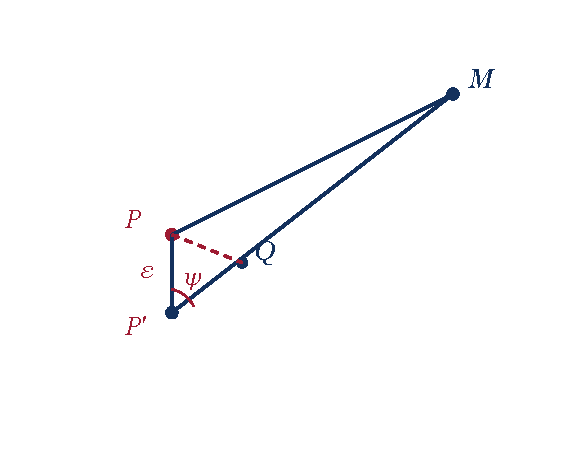
\includegraphics[width=0.55\textwidth]{figuras/pdf/cap04-fig1.pdf}
\caption{Potencial de la doble capa: los elementos correspondientes $P$ y
$P'$, de densidades $X_1$ y $-X_1$, separados por $\varepsilon$; el punto
$M$ y el ángulo $\psi$.}
\label{fig:cap4-1}
\end{figure}

Siendo arbitraria la función $X_1$, podremos, sin disminuir la generalidad
de la solución particular (9), reemplazar $X_1\varepsilon$ por una sola
letra $X_2$ que designe una función cualquiera de $x,y,z$. Además, puesto
que hemos puesto $F(r)=e^{i\alpha r}/r$, tendremos, para la derivada,
$F'(r)=\dfrac{e^{i\alpha r}}{r}\left(i\alpha-\dfrac1r\right)$. Por
consiguiente, la expresión (9) de $\xi_0$ puede escribirse
\begin{equation}
\xi_0 = \int X_2\,\frac{e^{i\alpha r}}{r}\left(i\alpha-\frac1r\right)
\cos\psi\,d\omega.
\tag{10}
\end{equation}
Pongamos aún: $\xi_0=\xi_1+\xi_2$,
\[
\xi_1 = -\int \frac{X_2\cos\psi}{r^2}\,d\omega,\qquad
\xi_2 = \int X_2\cos\psi\left[\frac{i\alpha e^{i\alpha r}}{r} -
\frac{e^{i\alpha r}}{r^2} + \frac{1}{r^2}\right]d\omega.
\]
Vemos que $\xi_1$ representa el potencial newtoniano de una doble capa. En
cuanto a la segunda integral $\xi_2$ (como la función bajo el signo $\int$
no se vuelve infinita), será continua, así como todas sus derivadas.

La teoría del potencial newtoniano nos enseña que $d\xi_1/dn$ es continua,
pero que $\xi_1$ es una función discontinua. Luego $d\xi_0/dn$ es continua
y $\xi_0$ será una función discontinua, que sufrirá un salto brusco igual
a $4\pi X_2$ al atravesar la superficie atrayente.

\noindent\textbf{81.} La combinación de las integrales (7) y (10) nos da
la solución más general de la ecuación (1).

En efecto, si $X_1$ y $X_2$ son dos funciones cualesquiera de las
coordenadas de un elemento $d\omega$ de una superficie cualquiera; si $r$
es la longitud de la recta que une el elemento $d\omega$ con el punto
$x,y,z$; y si $\psi$ designa el ángulo que forma esa recta con la normal
al elemento $d\omega$, la expresión
\begin{equation}
\xi_0 = \int X_1\frac{e^{i\alpha r}}{r}\,d\omega +
\int X_2\cos\psi\,\frac{e^{i\alpha r}}{r}\left(i\alpha-\frac1r\right)d\omega
\tag{11}
\end{equation}
satisfará la ecuación (1). Nos queda por mostrar que esa es, en efecto, la
integral general.

Sea $U$ una función cualquiera, finita y continua, así como todas sus
derivadas, y que satisface la ecuación (1) fuera de una cierta superficie
$S$.

Sea $V$ el potencial debido a un cierto volumen atrayente, cuya parte
podrá encontrarse fuera de la superficie $S$. Tendremos
\begin{equation}
\Delta V+\alpha^2V=0,
\tag{12}
\end{equation}
fuera del volumen atrayente, y en un punto de ese volumen
\begin{equation}
\Delta V+\alpha^2V+4\pi\rho=0,
\tag{13}
\end{equation}
siendo $\rho$ la densidad de la materia atrayente.

El teorema de Green nos da:
\begin{equation}
\int\left(U\frac{dV}{dn}-V\frac{dU}{dn}\right)d\omega =
\int(U\Delta V-V\Delta U)\,d\tau,
\tag{14}
\end{equation}
extendiéndose la primera integral a todos los elementos $d\omega$ de la
superficie $S$ y la segunda a todos los elementos de volumen $d\tau$ del
espacio exterior a esa superficie. En el cálculo de las derivadas
$dU/dn$ y $dV/dn$ se considera la normal al elemento $d\omega$ dirigida
hacia el interior de la superficie $S$.

Como $U$ satisface la ecuación (1) y $V$ las ecuaciones (12) y (13), la
integral del segundo miembro de (14) se reducirá a
\[
-4\pi\int U\rho\,d\tau,
\]
debiendo extenderse la integración al volumen atrayente que engendra el
potencial $V$, o más bien a la porción de ese volumen exterior a $S$.

Supongamos ahora que el volumen atrayente que engendra $V$ se reduzca a
una esfera de radio muy pequeño cuyo centro sea el punto $x_0,y_0,z_0$, y
que la densidad $\rho$ sea tal que la masa atrayente total sea igual a
$1$. Entonces, llamando $r_0$ a la distancia de un elemento $d\omega$ de
$S$ al punto $x_0,y_0,z_0$, el valor de $V$ en el centro de gravedad de
ese elemento se reducirá a $e^{i\alpha r_0}/r_0$ y el de $dV/dn$ a
$+\cos\psi\,\dfrac{e^{i\alpha r_0}}{r_0}\left(i\alpha-\dfrac{1}{r_0}\right)$,
designando siempre $\psi$ el ángulo de la normal exterior al elemento
$d\omega$ con la recta que une ese elemento con el punto $x_0,y_0,z_0$.

La integral $\int U\rho\,d\tau$ se reducirá a $U_0$ ($U_0$ el valor de $U$
en el punto $x_0,y_0,z_0$), si ese punto es exterior a $S$. Esta integral
es nula en el caso contrario, pues se extiende a la porción del volumen
atrayente exterior a $S$, y si el punto $x_0,y_0,z_0$ es interior a $S$,
lo mismo ocurre con todo el volumen atrayente. Se tiene, pues, simplemente:
\[
-4\pi U_0 = \int\left(U\frac{dV}{dn}-V\frac{dU}{dn}\right)d\omega.
\]
Si, suprimiendo los índices, llamamos $x,y,z$ al punto que llamábamos
$x_0,y_0,z_0$; $r$ a su distancia al elemento $d\omega$, y $U$ al valor de
la función $U$ en ese punto, resulta simplemente:
\begin{equation}
U = -\int \frac{U}{4\pi}\frac{e^{i\alpha r}}{r}\left(i\alpha-\frac1r\right)
\cos\psi\,d\omega + \int \frac{dU}{dn}\,\frac{e^{i\alpha r}}{4\pi r}\,d\omega.
\tag{15}
\end{equation}
Se ve así que $U$, que es una función cualquiera que satisface la
ecuación (1), es igual a la expresión (11), con tal de tomar, para la
función arbitraria $X_1$, el valor $\dfrac{dU}{4\pi\,dn}$ en el elemento
$d\omega$, y para la función arbitraria $X_2$, el valor $-U/4\pi$ en ese
mismo elemento.

\noindent\textbf{82.} La ecuación (15) es válida si el punto $x,y,z$ es
exterior a $S$. En caso contrario, el segundo miembro de esa ecuación se
reduce a $0$, pues acabamos de ver que, si $x_0,y_0,z_0$ es interior a
$S$, la integral $\int U\rho\,d\tau$ es nula.

Si en la expresión (11) las funciones arbitrarias $X_1$ y $X_2$ son
cualesquiera, esa expresión representará siempre, fuera de $S$, una
función $U$ que satisfará la ecuación (1); pero no ocurrirá, en general,
que $U$ se reduzca a $-4\pi X_2$ y $dU/dn$ a $4\pi X_1$ cuando el punto
$x,y,z$ se aproxime indefinidamente a un elemento $d\omega$ de $S$.

Para que así sea, es necesario, según lo que acabamos de ver, que la
expresión (11) sea nula cada vez que el punto $x,y,z$ sea interior a $S$.

Esta condición es suficiente. En efecto, si se cumple, en un punto
infinitamente vecino de $S$, pero interior a esa superficie, los valores
de la expresión (11) y de sus derivadas serán nulos.

Consideremos ahora un punto infinitamente vecino del primero, pero
exterior a $S$. Según lo que dijimos más arriba sobre la discontinuidad
del potencial de una capa simple o de una doble capa, los valores de $U$ y
de $dU/dn$ en esos dos puntos infinitamente vecinos deberán diferir en
cantidades iguales, respectivamente, a $4\pi X_1$ y $-4\pi X_2$.

Ahora bien, en el primer punto se tiene $U=dU/dn=0$. Tendremos, pues, en
el segundo,
\[
U=-4\pi X_2,\qquad \frac{dU}{dn}=4\pi X_1.
\]

\section{Ecuaciones de la difracción}

\noindent\textbf{83. Ecuaciones de la difracción.} — Sea $O$ una fuente
luminosa que supondremos reducida a un punto cuyos desplazamientos son
funciones periódicas del tiempo. Este punto se convertirá en el centro de
una serie de ondas esféricas, cada uno de cuyos puntos estará animado de
un movimiento periódico. Las componentes del desplazamiento de uno de
esos puntos serán las partes reales de expresiones de la
forma\footnote{Aquí el original reinicia su numeración de ecuaciones,
que ya había llegado a (15) en el §81; las ecuaciones (1) a (11) de los
§§83-94 no deben confundirse con las de los §§76-82 ni con las de los
§§95-99, que vuelven a empezar en (1) más adelante. Conservamos la
numeración de Poincaré.}
\begin{equation}
\xi=\xi_1e^{-i\alpha Vt},\qquad \eta=\eta_1e^{-i\alpha Vt},\qquad
\zeta=\zeta_1e^{-i\alpha Vt},
\tag{1}
\end{equation}
satisfaciendo $\xi_1,\eta_1,\zeta_1$ las ecuaciones diferenciales
\begin{equation}
\Delta\xi_1+\alpha^2\xi_1=0,\qquad \Delta\eta_1+\alpha^2\eta_1=0,\qquad
\Delta\zeta_1+\alpha^2\zeta_1=0,
\tag{2}
\end{equation}
\[
\Theta_1=\frac{d\xi_1}{dx}+\frac{d\eta_1}{dy}+\frac{d\zeta_1}{dz}=0.
\]
Las ondas son esféricas, de donde resulta, no que $\xi_1,\eta_1,\zeta_1$
sean funciones solo de $r$ (lo cual es incompatible con la condición de
transversalidad), sino que esas cantidades varían mucho más lentamente al
desplazarse sobre la superficie de una esfera $S$ con centro en $O$ que si
se desplaza normalmente a esa esfera.

Pondremos, pues,
\[
\xi_1=\xi_2e^{i\alpha r},\qquad \eta_1=\eta_2e^{i\alpha r},\qquad
\zeta_1=\zeta_2e^{i\alpha r},
\]
variando $\xi_2,\eta_2,\zeta_2$ mucho más lentamente que el factor
$e^{i\alpha r}$.

La derivada de $e^{i\alpha r}$ es igual a $i\alpha e^{i\alpha r}$; como
$\alpha=2\pi/\lambda$ es una cantidad muy grande, esta derivada es, a su
vez, muy grande. Por el contrario, supondremos que las derivadas de
$\xi_2,\eta_2,\zeta_2$ son cantidades finitas.

Sean $l,m,n$ los cosenos directores de la normal a la esfera $S$;
necesitamos $d\xi_1/dn=l\,d\xi_1/dx+m\,d\xi_1/dy+n\,d\xi_1/dz$.

Hallamos:
\[
\frac{d\xi_1}{dn}=\frac{d\xi_1}{dr}=i\alpha\xi_2e^{i\alpha r}+
\frac{d\xi_2}{dr}e^{i\alpha r}.
\]
El segundo término es muy pequeño frente al primero, porque $\alpha$ es
muy grande; se tiene, pues, aproximadamente $d\xi_1/dn=i\alpha\xi_1$; y,
del mismo modo, $d\eta_1/dn=i\alpha\eta_1$, $d\zeta_1/dn=i\alpha\zeta_1$.

Supongamos ahora que una porción de una esfera $S$ con centro en el punto
luminoso esté ocupada por una pantalla. La intensidad luminosa en un
punto del éter interior a la esfera será muy sensiblemente la misma que
si no existiera la pantalla. Lo mismo ocurrirá para los puntos de la
esfera exteriores a la pantalla. Para los puntos de la pantalla, la
intensidad debe ser muy sensiblemente nula.

\noindent\textbf{84.} He aquí, pues, las condiciones que tendremos que
cumplir:

Fuera de la esfera $S$, las tres componentes del desplazamiento serán las
partes reales de las exponenciales $\xi_0e^{-i\alpha Vt}$,
$\eta_0e^{-i\alpha Vt}$, $\zeta_0e^{-i\alpha Vt}$, y las funciones
$\xi_0,\eta_0,\zeta_0$ deberán satisfacer las cuatro condiciones
siguientes.

A. Se deberá tener, fuera de $S$,
$\Delta\xi_0+\alpha^2\xi_0=\Delta\eta_0+\alpha^2\eta_0=
\Delta\zeta_0+\alpha^2\zeta_0=0$.

B. En todos los puntos de $S$ que no pertenecen a la pantalla, se debe
tener muy sensiblemente
\[
\xi_0=\xi_1,\quad \frac{d\xi_0}{dn}=\frac{d\xi_1}{dn}=i\alpha\xi_1,\qquad
\eta_0=\eta_1,\quad \frac{d\eta_0}{dn}=\frac{d\eta_1}{dn}=i\alpha\eta_1,
\]
\[
\zeta_0=\zeta_1,\quad \frac{d\zeta_0}{dn}=\frac{d\zeta_1}{dn}=i\alpha\zeta_1.
\]

C. En todos los puntos de la pantalla se debe tener muy sensiblemente
\[
\xi_0=\eta_0=\zeta_0=\frac{d\xi_0}{dn}=\frac{d\eta_0}{dn}=
\frac{d\zeta_0}{dn}=0.
\]

D. Debe cumplirse la condición de transversalidad
$\Theta_0=d\xi_0/dx+d\eta_0/dy+d\zeta_0/dz=0$.

Es imposible satisfacer exactamente las condiciones B y C; solo se pueden
satisfacer muy sensiblemente, es decir, salvo cantidades del orden de la
longitud de onda $\lambda$.

Vimos más arriba que, si una función $\xi_0$ satisface la ecuación
$\Delta\xi_0+\alpha^2\xi_0=0$ fuera de una superficie $S$, y si en los
diversos puntos de esa superficie se reduce a $-4\pi X_2$ mientras
$d\xi_0/dn$ se reduce a $4\pi X_1$, se tendrá, fuera de $S$,
\begin{equation}
\xi_0 = \int X_2\,\frac{e^{i\alpha r}}{r}\left(i\alpha-\frac1r\right)
\cos\psi\,d\omega + \int X_1\,\frac{e^{i\alpha r}}{r}\,d\omega,
\tag{3}
\end{equation}
mientras que, dentro de $S$, el segundo miembro de (3) se reducirá a $0$.

Aquí nuestra superficie $S$ se reduce a una esfera con centro en $O$;
$\xi_0$ y $d\xi_0/dn$ son muy sensiblemente nulos para los puntos de la
pantalla; para los puntos exteriores a la pantalla, $\xi_0$ es
aproximadamente igual a $\xi_1$ y $d\xi_0/dn$ a $i\alpha\xi_1$ si se
considera la normal a $S$ dirigida hacia el exterior, y a $-i\alpha\xi_1$
si se considera esa normal dirigida hacia el interior, como se debe hacer
al aplicar la fórmula (15) del §81.

Si, pues, tomamos $X_1=i\alpha X_2=0$ para los puntos de la pantalla de
$S$, y $X_1=i\alpha X_2=-i\alpha\xi_1/4\pi$ para los puntos exteriores a
la pantalla, el segundo miembro de (3) diferirá muy poco de $\xi_0$ fuera
de $S$ y muy poco de $0$ dentro de $S$.

Llegamos, pues, a la siguiente conclusión.

Si existen funciones $\xi_0,\eta_0,\zeta_0$ que satisfagan
aproximadamente las condiciones A, B, C, D, esas funciones estarán muy
sensiblemente representadas por las integrales
\begin{gather}
\xi_0=\int X_2\,d\omega\,\frac{e^{i\alpha r}}{r}
\left(i\alpha+i\alpha\cos\psi-\frac{\cos\psi}{r}\right),\notag\\
\eta_0=\int Y_2\,d\omega\,\frac{e^{i\alpha r}}{r}
\left(i\alpha+i\alpha\cos\psi-\frac{\cos\psi}{r}\right),\tag{4}\\
\zeta_0=\int Z_2\,d\omega\,\frac{e^{i\alpha r}}{r}
\left(i\alpha+i\alpha\cos\psi-\frac{\cos\psi}{r}\right),\notag
\end{gather}
extendidas a todos los elementos $d\omega$ de la esfera $S$. En estas
fórmulas, $X_2=Y_2=Z_2=0$ si el elemento $d\omega$ pertenece a la
pantalla, y se tiene $X_2=-\xi_1/4\pi$, $Y_2=-\eta_1/4\pi$,
$Z_2=-\zeta_1/4\pi$ si el elemento $d\omega$ no pertenece a la pantalla.

\noindent\textbf{85.} Nos queda por mostrar que existen efectivamente funciones que satisfacen
esas condiciones; tenemos, pues, que mostrar que las expresiones (4)
cumplen muy aproximadamente las condiciones A, B, C, D.

$1^\circ$ La condición A se cumple ciertamente según lo dicho en el §82.

$2^\circ$ Según lo que vimos en ese mismo párrafo, las condiciones B y C
se cumplirían exactamente si las integrales (4) fueran exactamente nulas
dentro de $S$. Se cumplirán, pues, sensiblemente si esas integrales son
sensiblemente nulas dentro de $S$.

Tenemos, pues, que demostrar primero que las integrales (4) son
sensiblemente nulas dentro de $S$ y, para ello, dar un método para
calcular aproximadamente esas integrales. Es lo que haremos en el párrafo
siguiente.

Estableceremos después que, si $\xi_0,\eta_0,\zeta_0$ están definidas por
las fórmulas (4), se tiene muy sensiblemente
$\Theta_0=d\xi_0/dx+d\eta_0/dy+d\zeta_0/dz=0$.

Observemos de paso que las integrales (4) representan, dentro y fuera de
$S$, dos funciones distintas que no son la continuación analítica una de
la otra. Esto se debe a la discontinuidad del potencial de una capa
simple o de una doble capa. Por eso las integrales de Fresnel, que dan
cuenta de los fenómenos ópticos que ocurren fuera de la esfera $S$, no
representan los fenómenos que ocurren dentro de esa esfera. Esa es la
explicación de las anomalías señaladas por Poisson.

\section{Cálculo de las integrales}

\noindent\textbf{86. Cálculo de las integrales (4).} — Vamos a tratar de
calcular aproximadamente la primera integral (4), que escribiremos
\begin{equation}
\xi_0 = \int X\,\frac{e^{i\alpha r}}{r}\,d\omega,
\tag{5}
\end{equation}
poniendo, para abreviar,
\begin{equation}
X = X_2\left[i\alpha(1+\cos\psi)-\frac{\cos\psi}{r}\right].
\tag{6}
\end{equation}

Cambiemos de coordenadas. Siendo $S$
(figura~\ref{fig:cap4-2}) la esfera de la cual una porción está ocupada
por una pantalla, y $P$ el punto iluminado $x,y,z$, la posición de un
punto quedará determinada, en el nuevo sistema de coordenadas, por el
ángulo $\varphi$ que forma el plano que pasa por ese punto y la recta $OP$
con un plano fijo trazado por $OP$, por el ángulo $\theta$ de la recta que
une el punto con el punto $O$ con $OP$, y, por último, por el radio vector
$R$ trazado desde el punto $O$. En este sistema, un elemento de la
superficie de la esfera $S$ de radio $a$ tiene por expresión
\[
d\omega = a^2\sin\theta\,d\theta\,d\varphi.
\]

\begin{figure}[htbp]
\centering
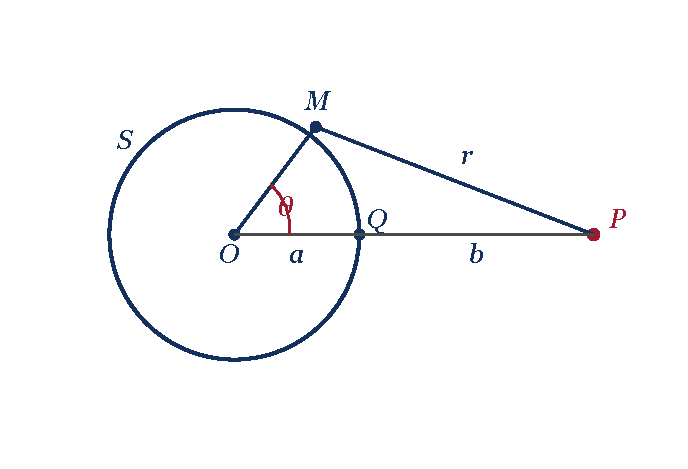
\includegraphics[width=0.7\textwidth]{figuras/pdf/cap04-fig2.pdf}
\caption{Cambio de coordenadas sobre la esfera $S$: el punto $M$, el
centro $O$, el polo $Q$ y el punto iluminado $P$.}
\label{fig:cap4-2}
\end{figure}

Se puede dar a esta expresión otra forma. Designando por $b$ la distancia
$QP$ del punto $P$ a la esfera, tenemos, en el triángulo $MOP$:
\[
r^2=(a+b)^2+a^2-2a(a+b)\cos\theta;
\]
diferenciando, se obtiene
\[
r\,dr = a(a+b)\sin\theta\,d\theta.
\]
Y, si reemplazamos en $d\omega$ el producto $\sin\theta\,d\theta$ por su
valor tomado de esta última expresión, resulta:
\[
d\omega = \frac{a^2r\,dr}{a(a+b)}\,d\varphi = \frac{a}{a+b}\,r\,dr\,d\varphi.
\]
Llevando este valor de $d\omega$ a la expresión (5) de $\xi_0$, obtenemos
\begin{equation}
\xi_0 = \frac{a}{a+b}\iint X\,e^{i\alpha r}\,dr\,d\varphi,
\tag{7}
\end{equation}
tomándose la integración entre $b$ y $2a+b$ para $r$, y entre $0$ y $2\pi$
para $\varphi$.

Sin embargo, no extenderemos la integración más que a la parte de la
esfera $S$ no ocupada por la pantalla; eso no cambiará en nada el
resultado, puesto que sobre la pantalla la función $X$ es nula.
Tendremos así la ventaja de que, en todo el campo de integración, la
función $X$ será continua y sus derivadas serán finitas, lo cual es
necesario para lo que sigue. En estas condiciones, los límites de la
integración respecto de $r$ no serán forzosamente $b$ y $2a+b$. Los
llamaremos $r_1$ y $r_2$.

Integremos primero respecto de $r$. Aplicando la regla de la integración
por partes, y designando por $r_1$ y $r_2$ los límites de la variable,
tendremos
\[
\int X\,e^{i\alpha r}\,dr =
\left[\frac{X\,e^{i\alpha r}}{i\alpha}\right]_{r_1}^{r_2}
-\frac{1}{i\alpha}\int\frac{dX}{dr}\,e^{i\alpha r}\,dr,
\]
y, si integramos por partes la integral del segundo miembro, obtendremos
\[
\int X\,e^{i\alpha r}\,dr =
\left[\frac{X\,e^{i\alpha r}}{i\alpha}\right]_{r_1}^{r_2}
+\frac{1}{\alpha^2}\left[\frac{dX}{dr}\,e^{i\alpha r}\right]_{r_1}^{r_2}
-\frac{1}{\alpha^2}\int\frac{d^2X}{dr^2}\,e^{i\alpha r}\,dr,
\]
siendo $\alpha$ una cantidad infinitamente grande, podemos en general, en
el cálculo aproximado que nos hemos propuesto, despreciar los términos del
segundo miembro que contienen como factor una potencia de $\alpha$
inferior a $-1$. Tenemos entonces
\[
\int X\,e^{i\alpha r}\,dr =
\left[\frac{X\,e^{i\alpha r}}{i\alpha}\right]_{r_1}^{r_2},
\]
y el valor de $\xi_0$ dado por la integral (7) es, aproximadamente,
\begin{equation}
\xi_0 = \frac{a}{a+b}\int_0^{2\pi}
\left[\frac{X\,e^{i\alpha r}}{i\alpha}\right]_{r_1}^{r_2} d\varphi.
\tag{8}
\end{equation}

\noindent\textbf{87.} En la figura~\ref{fig:cap4-2}, el punto $P$ se
encuentra fuera de la esfera $S$; pero es evidente que, si hubiéramos
tomado el punto $P$ dentro de la esfera, habríamos llegado a la misma
expresión de $\xi_0$ considerando, en ese caso, como negativa la distancia
$b$ del punto a la esfera.

Vamos a mostrar, con ayuda de la expresión (8), que el valor de $\xi_0$ es
sensiblemente nulo en un punto interior a la esfera.

Veamos, en efecto, qué representan los límites superior e inferior $r_1$
y $r_2$. Pueden presentarse varios casos; solo consideraremos tres:

$1^\circ$ No hay pantalla. Se tiene entonces $r_1=b$, $r_2=2a+b$, si el
punto $P$ es exterior a la esfera, y $r_1=b$, $r_2=2a-b$, si el punto $P$
es interior a la esfera.

$2^\circ$ Hay una pantalla; el punto $Q$, polo del punto $P$, no está en
la pantalla, pero el punto diametralmente opuesto pertenece a ella.

Entonces $r_1=b$; y el límite superior $r_2$, que es en general una
función de $\varphi$, es el valor de $r$ que corresponde al borde de la
pantalla.

$3^\circ$ Hay una pantalla; el punto $Q$ pertenece a la pantalla, y el
punto diametralmente opuesto no forma parte de ella.

Entonces $r_2=2a\pm b$ y $r_1$ es el valor de $r$ que corresponde al borde
de la pantalla.

Llamemos $J$ a la integral $\displaystyle\int_0^{2\pi}
\dfrac{X\,e^{i\alpha r}}{i\alpha}\,d\varphi$ tomada a lo largo del borde
de la pantalla, y sean $X'$ y $X''$ los valores de
$\dfrac{X\,e^{i\alpha r}}{i\alpha}$ en el punto $Q$ y en el punto
diametralmente opuesto.

Tendremos: en el primer caso,
$\xi_0=\dfrac{a}{a+b}(2\pi X''-2\pi X')$; en el segundo,
$\xi_0=\dfrac{a}{a+b}(J-2\pi X')$; en el tercero,
$\xi_0=\dfrac{a}{a+b}(2\pi X''-J)$.

Veremos más adelante que $J$ es generalmente despreciable.

Nos queda por calcular $X'$ y $X''$. Tenemos
$X=X_2\left(i\alpha+i\alpha\cos\psi-\dfrac{\cos\psi}{r}\right)$. El
último término $\cos\psi/r$ es despreciable frente a $i\alpha$ porque
$\alpha$ es muy grande. Queda, pues,
$X=i\alpha X_2(1+\cos\psi)=-\dfrac{i\alpha\xi_1}{4\pi}(1+\cos\psi)$,
puesto que, fuera de la pantalla, $X_2$ es igual a $-\xi_1/4\pi$.

En el punto $Q$ se tiene: si el punto $P$ es exterior a $S$, $\psi=0$,
$X'=-\dfrac{\xi_1}{2\pi}e^{i\alpha b}$; si el punto $P$ es interior a $S$,
$\psi=\pi$, $X'=0$.

En el punto diametralmente opuesto se tiene, en todos los casos, $\psi=\pi$
y $X''=0$.

Por consiguiente, si el punto $P$ es interior a $S$, la integral (8) será
generalmente despreciable.

\noindent\textbf{88.} Si el punto $P$ es exterior a $S$, se tiene, en los
tres casos considerados más arriba:

En el primer caso, $\xi_0=\xi_1e^{i\alpha b}\dfrac{a}{a+b}$.

En el segundo caso, $\xi_0=\xi_1e^{i\alpha b}\dfrac{a}{a+b}$.

En el tercer caso, $\xi_0=0$.

Luego, si el punto $Q$ no pertenece a la pantalla, es decir, si $P$ no
está en la sombra geométrica, la intensidad es la misma que si no hubiera
pantalla. Si, por el contrario, $P$ está en la sombra geométrica, la
intensidad es nula. En otras palabras, los fenómenos son los mismos que
en la teoría geométrica de las sombras. No habrá, pues, fenómenos de
difracción sino cuando la integral $J$ no sea despreciable.

Nos vemos, pues, llevados a: $1^\circ$ demostrar que la integral $J$ es
generalmente despreciable; $2^\circ$ buscar cuáles son los casos de
excepción en que deja de serlo.

Tenemos que evaluar la integral
$J=\displaystyle\int \dfrac{X\,e^{i\alpha r}}{i\alpha}\,d\varphi$
extendida a todo el contorno de la pantalla.

Para ello descompondremos ese contorno en cierto número de arcos
parciales, que serán de dos clases:

$1^\circ$ sobre los arcos de la primera clase, la derivada $d\varphi/dr$
será finita;

$2^\circ$ sobre los arcos de la segunda clase, esa derivada será lo
bastante grande como para no ser despreciable frente a $\alpha$.

Por lo demás, nada nos impide suponer que la subdivisión del contorno en
arcos parciales se ha hecho de tal modo que, a lo largo de cada uno de
esos arcos, $r$ sea constantemente creciente o constantemente decreciente.

\noindent\textbf{89.} Evaluemos primero la integral tomada a lo largo de
un arco de la primera clase.

Si tomamos como variable de integración $r$, nuestra integral se escribirá:
\[
\int \frac{X\,e^{i\alpha r}}{i\alpha}\,\frac{d\varphi}{dr}\,dr.
\]
Integrando por partes, se tiene
\[
-\frac{X\,e^{i\alpha r}}{\alpha^2}\,\frac{d\varphi}{dr}
+\frac{1}{\alpha^2}\int e^{i\alpha r}\,\frac{d}{dr}
\left(X\,\frac{d\varphi}{dr}\right)dr.
\]
Ahora bien, $X$ es del mismo orden que $\alpha$; si, pues, $d\varphi/dr$
es una cantidad finita, cada uno de los términos de esta última suma es
del orden de $1/\alpha$, es decir, despreciable. Así, la integral tomada a
lo largo de un arco de la primera clase es despreciable.

La integral $\displaystyle\int_{\varphi_0}^{\varphi_1}
\dfrac{X\,e^{i\alpha r}}{i\alpha}\,d\varphi$ tomada a lo largo de un arco
de la segunda clase será también despreciable en general, porque la
diferencia $\varphi_1-\varphi_0$ de los límites de integración será del
mismo orden de magnitud que $1/\alpha$.

Para que la integral $J$ tenga un valor finito, es necesario, pues, que
$\varphi_1-\varphi_0$ sea finito, es decir, que al menos uno de los arcos
de la segunda clase sea visto desde el punto $Q$ bajo un ángulo finito; lo
cual puede ocurrir en dos casos:

$1^\circ$ si ese arco es en sí mismo finito; se tiene entonces, a lo largo
de todo ese arco, $d\varphi/dr=\infty$, $dr/d\varphi=0$, $r=\text{const.}$;
es decir, que el arco en cuestión debe diferir muy poco de un arco de
círculo con polo en $Q$.

$2^\circ$ si ese arco pasa muy cerca del punto $Q$, es decir, si ese punto
está muy próximo al borde de la pantalla.

Cada vez que no sea así, la integral $J$ será despreciable y no tendremos
otros fenómenos que los previstos por la teoría geométrica de las
sombras.

\noindent\textbf{90.} Busquemos, pues, en qué casos $d\varphi/dr$ es
infinito. Hallamos en el §86 $r\,dr=a(a+b)\sin\theta\,d\theta$; de donde
deducimos\footnote{En el original no hay ninguna ecuación numerada (9)
en esta serie: la numeración pasa directamente de la (8) del §86 a la
(10). Conservamos la numeración de Poincaré.}
\begin{equation}
\frac{d\varphi}{dr} = \frac{1}{a(a+b)}\,\frac{r}{\sin\theta}\,
\frac{d\varphi}{d\theta}.
\tag{10}
\end{equation}
Esta igualdad nos muestra que $d\varphi/dr$ podrá volverse infinita en dos
casos: $1^\circ$ si $\sin\theta$ es muy pequeño; $2^\circ$ si
$d\varphi/d\theta$ es infinito.

Consideremos el primer caso. Siendo muy pequeño el ángulo $\theta$, un
arco del contorno de la pantalla está muy próximo al punto $Q$, y se puede
confundir la porción de la esfera que contiene ese arco con un plano que
pase por $Q$. Además, siendo infinitamente pequeño ese arco, se le puede
considerar como un elemento de una recta $AB$ (figura~\ref{fig:cap4-3}).
La distancia del punto $Q$ al elemento de arco $M$ es $a\theta$, siendo
$a$ el radio de la esfera sobre la que se encuentra la porción
considerada del contorno de la pantalla. Llamando $a\delta$ a la distancia
más corta $QC$ del punto $Q$ a la recta $AB$, y $\varphi$ al ángulo de
$QM$ y $QC$, tenemos
\[
a\theta\cos\varphi = a\delta \qquad\text{o bien}\qquad \theta\cos\varphi=\delta.
\]

\begin{figure}[htbp]
\centering
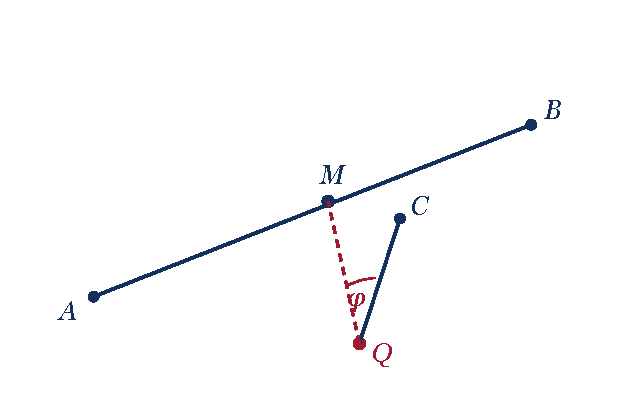
\includegraphics[width=0.6\textwidth]{figuras/pdf/cap04-fig3.pdf}
\caption{El arco del borde de la pantalla, confundido con la recta $AB$
cerca del polo $Q$; distancia $QC=a\delta$ y ángulo $\varphi$.}
\label{fig:cap4-3}
\end{figure}

El ángulo $\varphi$ que consideramos aquí no difiere, por lo demás, más
que en una constante del ángulo designado antes con la misma letra; sus
diferenciales tendrán, pues, el mismo valor. Diferenciando los dos
miembros de la igualdad anterior, hallamos
\[
\frac{d\theta}{d\varphi}\cos\varphi - \theta\sin\varphi = 0,
\]
nueva igualdad que nos muestra que $d\theta/d\varphi$ es del mismo orden
que $\theta$, y por tanto que $\delta$. Por consiguiente, $d\varphi/d\theta$
es del orden de $1/\delta$, y $d\varphi/dr$, dado por la relación (10), es
del orden de $r/\delta^2$.

Si el punto $P$ está a una distancia finita $r$ de la esfera, $d\varphi/dr$
es del orden de $1/\delta^2$, y, si se quiere que esta derivada sea del
mismo orden que $1/\lambda$, es necesario que $\delta$ sea del orden de
$\sqrt{\lambda}$. Si, por el contrario, el punto $P$ está a una distancia
de la esfera del orden de $\lambda$, será necesario que $\delta$ sea del
mismo orden que $\lambda$ para que $d\varphi/dr$ sea un infinito del orden
de $1/\lambda$.

La recta que une el punto $P$ con la fuente luminosa deberá, pues,
encontrar la esfera a una distancia del contorno de la pantalla del orden
de $\lambda$ para que haya en $P$ una iluminación anómala; la región en
que debe hallarse el punto $P$ es entonces demasiado pequeña para ser
observable. No se podrán observar anomalías en la iluminación de $P$ sino
cuando este se halle a una distancia finita de la esfera.

Así, sobre una esfera concéntrica a $S$, de radio $a+b$, siendo $b$
finito, la región ocupada por las franjas de difracción es del mismo
orden de magnitud que $\sqrt{\lambda}$. Sobre la esfera $S$ misma, esa
región es del mismo orden de magnitud que $\lambda$.

\noindent\textbf{91.} Examinemos el segundo caso, en el cual $d\varphi/dr$
es una cantidad infinitamente grande; siendo infinito $d\theta/d\varphi$,
$d\varphi/d\theta$ debe ser infinitamente pequeño. Si, pues, $r/\sin\theta$
es una cantidad finita, será necesario, para que $d\varphi/dr$ sea del
orden de $1/\lambda$, que $d\theta/d\varphi$ sea del orden de $\lambda$.

Es necesario, en otros términos, que $\theta$ sea constante salvo
cantidades del orden de $\lambda$, es decir que, despreciando las
cantidades de ese orden, un arco finito del contorno de la pantalla pueda
considerarse como un arco de círculo con centro en $Q$; la distancia del
punto $Q$ al centro de curvatura medio de ese arco debe ser, pues, del
orden de $\lambda$; de ahí resulta que los puntos iluminados de manera
anómala están todos contenidos dentro de un círculo cuyo radio es del
orden de $\lambda$, y que los fenómenos son inobservables.

Es necesario, pues, para que la observación sea posible, que $\sin\theta$,
y por consiguiente el radio de ese arco de círculo, sean muy pequeños.

Si $\sin\theta/r$ es una cantidad del orden de $\sqrt{\lambda}$, bastará
que $d\theta/d\varphi$ sea del orden de $\lambda$, y, por tanto, que la
distancia del punto $Q$ al centro del arco de círculo sea también del
mismo orden.

La región del espacio en la que debe situarse el punto $P$ para presentar
fenómenos anómalos es entonces lo bastante grande como para poder
observar esos fenómenos.

Observemos que, si el punto $P$ está situado sobre la esfera, su
iluminación quedará determinada por la teoría geométrica de las sombras,
o al menos la observación será incapaz de detectar una diferencia entre
la iluminación así determinada y la iluminación real.

Se tendrá, en efecto, cuando el punto $P$ tiende al punto $Q$,
$\sin\theta/r=1/a$, pues, en el triángulo $MOP$, se tiene
$\sin\theta/r=\sin OMP/a$, y en el límite el ángulo $OMP$ es recto. Siendo
finito $\sin\theta/r$, resultará aún, según lo que acabamos de ver, que
los fenómenos no serán observables.

\noindent\textbf{92.} Vamos a mostrar ahora que la condición de
transversalidad $\Theta_0=\xi_0'+\eta_0'+\zeta_0'=0$ se cumple para los
puntos $P$ situados fuera de la esfera $S$, o sobre esa misma esfera.

En efecto, $\Theta_0$ satisface la ecuación $\Delta\Theta_0+\alpha^2\Theta_0=0$.

Tenemos, pues, fuera de la esfera $S$, según el §81,
\[
\Theta_0 = -\int \frac{\Theta_0}{4\pi}\,\frac{e^{i\alpha r}}{r}
\left(i\alpha-\frac1r\right)\cos\psi\,d\omega +
\int \frac{1}{4\pi}\,\frac{d\Theta_0}{dn}\,\frac{e^{i\alpha r}}{r}\,d\omega,
\]
extendiéndose las integrales del segundo miembro a todos los elementos
$d\omega$ de la esfera $S$.

Ahora bien, vimos que, dejando de lado la región en que hay franjas de
difracción, los fenómenos son los mismos que en la teoría geométrica de
las sombras; en otras palabras, la iluminación es nula en ciertos puntos
y en otros es la misma que si no hubiera pantalla. En ambos casos,
$\Theta_0$ y $d\Theta_0/dn$ son nulos.

Bastará, pues, con el grado de aproximación adoptado, extender las
integrales del segundo miembro a la región de la esfera $S$ ocupada por
las franjas; ahora bien, vimos que esa región es del orden de $\lambda$.
Las integrales del segundo miembro son, pues, despreciables, y, por
consiguiente, lo mismo ocurre con $\Theta_0$.

En resumen, las integrales (4) satisfacen bien las condiciones A, B, C, D,
y no puede haber iluminación anómala sino cuando el punto $P$ está muy
próximo al borde de la sombra geométrica.

\noindent\textbf{93. Simplificación de las expresiones $\xi_0,\eta_0,\zeta_0$.}
— Vimos que, si el punto $Q$ está a una distancia finita de los bordes de
una pantalla, la iluminación del punto $P$ es la misma que en la teoría de
las sombras, y, en segundo lugar, que la iluminación se modifica si el
punto $Q$ está a una distancia de la pantalla del orden de $\sqrt{\lambda}$.
La iluminación de un punto no depende, pues, apenas más que de las
porciones de la esfera vecinas al punto $Q$. Este punto se llama el
\emph{polo} del punto $P$. Vamos a aprovechar esta observación para
simplificar los valores de $\xi_0,\eta_0,\zeta_0$ dados por las
integrales (4).

Tomemos la primera de esas integrales,
\[
\xi_0 = \int X_2\,d\omega\,\frac{e^{i\alpha r}}{r}
\left(i\alpha+i\alpha\cos\psi-\frac{\cos\psi}{r}\right).
\]
Puesto que las partes de esta integral que no son despreciables son las
que corresponden a los puntos muy próximos al polo $Q$ del punto iluminado
$P$, no extenderemos la integral sino a esos puntos, y podremos considerar
$X_2$ y $\psi$ como constantes. Como, además, $\alpha$ es una cantidad muy
grande y $r$ debe ser finito para que los fenómenos de difracción sean
observables, podemos, en la cantidad colocada bajo el signo de
integración, despreciar el término $\cos\psi/r$ frente a los otros dos
términos $i\alpha$ y $i\alpha\cos\psi$. Haciendo esta simplificación, y
sacando fuera de la integral los términos considerados como constantes,
tenemos
\[
\xi_0 = X_2\,i\alpha(1+\cos\psi)\int \frac{e^{i\alpha r}}{r}\,d\omega.
\]
Se sabe, por lo demás (§84), que $X_2=-\xi_1/4\pi$; por consiguiente,
reemplazando, en la expresión de $\xi_0$, $X_2$ y $\cos\psi$ por los
valores de esas cantidades en el polo $Q$, tendremos
\[
\xi_0 = -\frac{i\alpha}{2\pi}\,\xi_1 \int \frac{e^{i\alpha r}}{r}\,d\omega.
\]
La distancia $r$ del punto $P$ a los puntos de la esfera que están
próximos al polo $Q$ difiere muy poco de la distancia $PQ=b$, y, por
tanto, puede sacarse fuera de la integral, puesto que esta no se extiende
más que a los puntos vecinos de $Q$. El valor de $\xi_0$ se convertirá en
\[
\xi_0 = -\frac{i\alpha}{2\pi}\,\frac{\xi_1}{b}\int e^{i\alpha r}\,d\omega,
\]
y por último, mediante una última transformación,
\[
\xi_0 = -\frac{i\alpha\xi_1e^{i\alpha b}}{2\pi b}
\int e^{i\alpha(r-b)}\,d\omega.
\]

\noindent\textbf{94.} Busquemos el valor de esta última integral. Tenemos,
en el triángulo $MOP$ (figura~\ref{fig:cap4-2}),
$r^2=(a+b)^2+a^2-2a(a+b)\cos\theta$; y, como solo tenemos que considerar
puntos vecinos del polo $Q$, para los cuales $\theta$ es muy pequeño,
podemos reemplazar $\cos\theta$ por los dos primeros términos
$1-\theta^2/2$ de su desarrollo; tendremos
$r^2=(a+b)^2+a^2-2a(a+b)(1-\theta^2/2)$, o bien
$r^2=(a+b-a)^2+a(a+b)\theta^2=b^2+a(a+b)\theta^2$.

Designando por $s$ el arco de círculo máximo $QM$ comprendido entre un
punto $M$ de la esfera y el polo $Q$, tendremos $\theta\approx s/a$; y,
llevando este valor de $\theta$ a la expresión de $r^2$, resultará
$r^2=b^2+\dfrac{a+b}{a}s^2$. De ahí se obtiene,
$r-b=\dfrac{a+b}{a(r+b)}s^2$.

Pero, difiriendo $r$ muy poco de $b$, se puede reemplazar $r+b$ por $2b$,
de modo que se tiene $r-b=\dfrac{a+b}{2ab}s^2$.

Este valor de $r-b$, llevado a la expresión de $\xi_0$, da
\[
\xi_0 = -\frac{i\alpha\xi_1e^{i\alpha b}}{2\pi b}
\int e^{i\alpha\frac{a+b}{2ab}s^2}\,d\omega.
\]
No debiendo extenderse la integral más que a las porciones de la esfera
que rodean al punto $Q$, se pueden considerar esas porciones situadas en
el plano tangente a la esfera en $Q$. Tomemos, en ese plano, dos ejes de
coordenadas rectangulares que se cortan en $Q$. En este sistema, las
coordenadas del punto $M$ serán las distancias $l$ y $l'$ de ese punto a
los ejes. Para simplificar la expresión de $\xi_0$, definiremos la
posición del punto $M$ mediante dos parámetros $u$ y $v$ tales que
\[
l=u\sqrt{\frac{ab\lambda}{2(a+b)}},\qquad
l'=v\sqrt{\frac{ab\lambda}{2(a+b)}}.
\]
Se tiene entonces $s^2=l^2+l'^2=(u^2+v^2)\dfrac{ab\lambda}{2(a+b)}$, y
$d\omega=dl\,dl'=du\,dv\,\dfrac{ab\lambda}{2(a+b)}$.

Llevando estos valores de $s^2$ y de $d\omega$ a la expresión de $\xi_0$,
tendremos, tras las simplificaciones,
\[
\xi_0 = -\frac{i\alpha\xi_1a\lambda e^{i\alpha b}}{4\pi(a+b)}
\int e^{\frac14 i\alpha\lambda(u^2+v^2)}\,du\,dv,
\]
y, como habíamos puesto $\alpha=2\pi/\lambda$, obtenemos, reemplazando
$\alpha$ por ese valor,
\begin{equation}
\xi_0 = -\frac{ia\xi_1e^{i\alpha b}}{2(a+b)}
\int e^{\frac{i\pi}{2}(u^2+v^2)}\,du\,dv.
\tag{11}
\end{equation}

\section{Intensidad luminosa en un punto}

\noindent\textbf{95. Intensidad luminosa en un punto.} — Según lo dicho en
el §76, la componente según el eje $x$ del desplazamiento de un punto $P$
situado fuera de la esfera $S$ es $\xi=$ parte real de $\xi_0e^{-i\alpha Vt}$,
donde $\xi_0$ se reemplaza por la expresión (11) que acabamos de hallar.
Tendríamos para las otras dos componentes las cantidades
$\eta=$ parte real de $\eta_0e^{-i\alpha Vt}$,
$\zeta=$ parte real de $\zeta_0e^{-i\alpha Vt}$, deduciéndose $\eta_0$ y
$\zeta_0$ de $\xi_0$ al reemplazar, en la expresión (11), $\xi_1$ por
$\eta_1$ o $\zeta_1$. La intensidad luminosa en el punto $P$ será, pues,
proporcional a
$\rho\!\left[\!\left(\dfrac{d\xi}{dt}\right)^2+\!
\left(\dfrac{d\eta}{dt}\right)^2+\!\left(\dfrac{d\zeta}{dt}\right)^2\right]$;
ahora bien, se tiene
\[
\frac{d\xi}{dt} = \text{parte real de }
\left(-i\alpha V\xi_0e^{-i\alpha Vt}+e^{-i\alpha Vt}\frac{d\xi_0}{dt}\right)
\]
y dos expresiones análogas para $d\eta/dt$ y $d\zeta/dt$. Por
consiguiente, la intensidad es proporcional a la suma de los cuadrados de
los módulos de las tres cantidades análogas a
$\left(-i\alpha V\xi_0+\dfrac{d\xi_0}{dt}\right)$.

Pero, en el valor (11) de $\xi_0$, la única cantidad que depende del
tiempo es $\xi_1$, de modo que la intensidad es igual a la suma de los
cuadrados de los módulos de tres cantidades, de las cuales la
primera es\footnote{El original inicia aquí la tercera serie de numeración
de ecuaciones del capítulo; las (1) a (7) de los §§95-99 no
deben confundirse con las de los §§76-82 ni con las de los §§83-94.
Conservamos la numeración de Poincaré.}
\begin{equation}
\left(-i\alpha V\xi_1+\frac{d\xi_1}{dt}\right)
\frac{ia\,e^{i\alpha b}}{2(a+b)}
\int e^{\frac{i\pi}{2}(u^2+v^2)}\,du\,dv,
\tag{1}
\end{equation}
y de las cuales las otras dos se deducen de esta reemplazando $\xi_1$ por
$\eta_1$ y $\zeta_1$.

Observándose los fenómenos de difracción en un plano, tenemos que
considerar la intensidad relativa de los puntos situados en un mismo
plano. Estando esos puntos siempre vecinos entre sí y a cierta distancia
de la pantalla, podemos admitir que las distancias $b$ de cada uno de
ellos a la esfera que contiene la pantalla son las mismas. De ello
resulta que, en cada uno de los términos (1), cuya suma de cuadrados es
proporcional a la intensidad, el factor $\dfrac{ia\,e^{i\alpha b}}{2(a+b)}$
es el mismo para esos puntos, si solo se considera luz homogénea. Además,
como esos puntos se observan en el mismo instante y los valores de
$\xi_1,\eta_1,\zeta_1$ varían poco al pasar de un punto de la esfera $S$ a
un punto vecino, el factor $\left(-i\alpha V\xi_1+\dfrac{d\xi_1}{dt}\right)$
tendrá sensiblemente el mismo valor. La intensidad relativa de la luz en
los distintos puntos observados será, pues, proporcional, en el mismo
instante, al cuadrado del módulo de la integral,
\begin{equation}
\int e^{\frac{i\pi}{2}(u^2+v^2)}\,du\,dv,
\tag{2}
\end{equation}
que aparece como factor en el término (1) y en los dos que de él se
deducen. Nos bastará, pues, para hallar la intensidad luminosa en los
diversos puntos del plano donde se hacen las observaciones, estudiar las
variaciones del módulo de esta integral.

\section{Expresión de la integral en el caso de una rendija de bordes
paralelos}

\noindent\textbf{96. Expresión de la integral (2) en el caso de una
rendija de bordes paralelos.} — Supondremos que uno de los ejes a los que
corresponden los parámetros $u$ y $v$ sea paralelo a los bordes de la
rendija; sea ese el eje de las $u$, por ejemplo. Si nos remitimos a la
relación $\delta=u\sqrt{\dfrac{ab\lambda}{2(a+b)}}$, que liga el parámetro
$u$ con la distancia $\delta$ de un punto del plano $uv$ al eje de las
$v$, se ve que $u$ es del orden de $\delta/\sqrt{\lambda}$. Teniendo la
rendija una longitud, si no ilimitada, al menos muy grande respecto de las
cantidades del orden de $\sqrt{\lambda}$, los valores de $u$ serán siempre
muy grandes para los puntos que se observan. Por consiguiente, se pueden,
en la integral (2), considerar como infinitos los límites de $u$.
Designaremos por $v_1$ y $v_2$ los límites de $v$, que tienen en general
valores finitos, siendo pequeña la anchura de la rendija. Podemos poner
esta integral, cuyos límites son constantes, bajo la forma
\[
\int_{-\infty}^{+\infty} e^{\frac{i\pi}{2}u^2}\,du
\int_{v_1}^{v_2} e^{\frac{i\pi}{2}v^2}\,dv.
\]
La primera de estas integrales tiene por valor $1+i$, cuyo módulo es
$2$\footnote{Así en el original. El módulo de $1+i$ es $\sqrt2$; es su
cuadrado, que es lo que interviene en la intensidad, el que vale $2$.};
de modo que solo tenemos que ocuparnos de la segunda, que se convierte,
cuando se reemplaza en ella la exponencial por las funciones
trigonométricas, en
\begin{equation}
\int_{v_1}^{v_2} e^{\frac{i\pi}{2}v^2}\,dv =
\int_{v_1}^{v_2}\cos\frac{\pi v^2}{2}\,dv +
i\int_{v_1}^{v_2}\sin\frac{\pi v^2}{2}\,dv.
\tag{3}
\end{equation}

\section{Representación gráfica de la integral de Fresnel}

\noindent\textbf{97. Representación gráfica de la integral (3).} — Las
dos integrales del segundo miembro son conocidas con el nombre de
\emph{integrales de Fresnel}; vamos a estudiarlas. Para simplificar los
cálculos, supondremos nulo el límite inferior de estas integrales; será
fácil después pasar al caso general, en que los límites son cualesquiera,
tomando la suma algebraica de dos integrales de las cuales uno de los
límites es $0$.

Pongamos, pues,
\[
x=\int_0^v \cos\frac{\pi v^2}{2}\,dv,\qquad
y=\int_0^v \sin\frac{\pi v^2}{2}\,dv,
\]
y construyamos la curva lugar geométrico de los puntos de coordenadas $x$
e $y$. Pasa por el origen de coordenadas, pues se tiene $x=y=0$ para
$v=0$. Si se cambia $v$ por $-v$, el elemento de las integrales no
cambia, pero el límite superior cambia de signo, y $x$ e $y$ cambian a la
vez de signo; el origen es, pues, un centro de simetría de la curva.

Tomemos las diferenciales de $x$ y de $y$: tenemos
$dx=\cos\dfrac{\pi v^2}{2}\,dv$, $dy=\sin\dfrac{\pi v^2}{2}\,dv$. Elevando
al cuadrado y sumando, obtenemos $dx^2+dy^2=ds^2=dv^2$; luego $ds=dv$,
siendo $ds$ un elemento de arco de la curva. Integrando los dos miembros
de esta igualdad y tomando $0$ como constante de integración, lo cual
equivale a contar los arcos a partir del origen, puesto que $x=y=0$ para
$v=0$, se tiene $s=v$.

El cociente $dy/dx$ da la tangente del ángulo formado por el eje de las
$x$ y la tangente a la curva en el punto $x,y$; designando por $\omega$
ese ángulo,\footnote{Poincaré designa este ángulo por $\alpha$; lo
llamamos $\omega$ para no confundirlo con $\alpha=2\pi/\lambda$.} tenemos
\begin{equation}
\omega = \frac{\pi}{2}v^2.
\tag{4}
\end{equation}
El radio de curvatura en un punto viene dado por
$\dfrac{ds}{d\omega}=\dfrac{dv}{\pi v\,dv}=\dfrac{1}{\pi v}$; en el
origen, es decir, para $v=0$, el radio de curvatura es infinito, y, como
$\omega$ es nulo a la vez que $v$, el eje de las $x$ es una tangente de
inflexión en el punto $O$ (figura~\ref{fig:cap4-4}).

\begin{figure}[htbp]
\centering
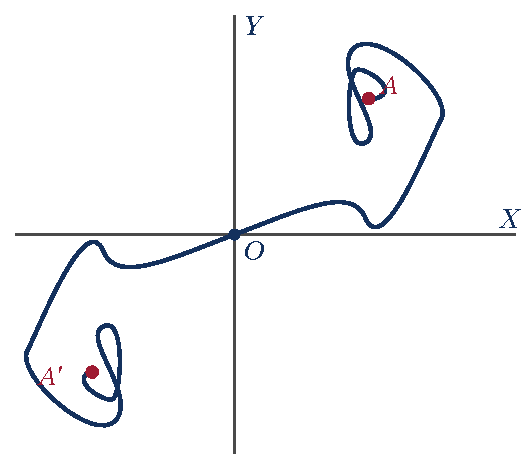
\includegraphics[width=0.7\textwidth]{figuras/pdf/cap04-fig4.pdf}
\caption{La espiral de Fresnel: la curva de coordenadas $x=\int_0^v
\cos(\pi v^2/2)\,dv$, $y=\int_0^v\sin(\pi v^2/2)\,dv$, con sus dos puntos
asintóticos $A$ y $A'$.}
\label{fig:cap4-4}
\end{figure}

Para construir la curva, haremos variar $v$ de $0$ a infinito; el ángulo
$\omega$ de la tangente a la curva con el eje $ox$ aumentará más allá de
todo límite; el radio de curvatura tenderá a $0$. Tendremos, pues, una
curva en forma de caracol, con un punto asintótico. Busquemos las
coordenadas de ese punto $A$. Para ello, busquemos el valor de la
integral $\displaystyle\int_0^\infty e^{\frac{i\pi}{2}v^2}\,dv$.

Se sabe que se tiene $\displaystyle\int_0^\infty e^{-z^2}\,dz=\frac12\sqrt\pi$.

Si ponemos $z^2=-\dfrac{i\pi}{2}v^2$, tenemos $z=v\sqrt{-i\pi/2}$,
$dz=dv\sqrt{-i\pi/2}$.

Por consiguiente, tendremos, para la integral buscada,
\[
\int_0^\infty e^{\frac{i\pi}{2}v^2}\,dv =
\frac12\sqrt\pi\,\sqrt{-\frac{2}{i\pi}} = \frac12\sqrt{2i} = \frac{1+i}{2};
\]
ahora bien, $\displaystyle\int_0^v e^{\frac{i\pi}{2}v^2}\,dv=x+iy$, luego,
para $v=\infty$, tenemos $x=\dfrac12$, $y=\dfrac12$.

Tales son las coordenadas del punto asintótico $A$. Se obtendrá la parte
de la curva correspondiente a valores negativos de $v$ por simetría.

\noindent\textbf{98.} Para definir mejor la curva, podemos buscar cómo
varía la distancia $AM$ del punto asintótico $A$ a un punto cualquiera $M$
de la parte de la curva correspondiente a los valores positivos de $v$.

Sea $v$ el valor del parámetro correspondiente a ese punto; sus
coordenadas serán $x=\int_0^v\cos(\pi v^2/2)\,dv$,
$y=\int_0^v\sin(\pi v^2/2)\,dv$.

Traslademos el origen de los ejes de coordenadas al punto $M$; la
abscisa del punto asintótico $A$ respecto de estos nuevos ejes será igual
a su abscisa respecto de los antiguos ejes, disminuida en la abscisa del
punto $M$, es decir,
\[
\int_0^\infty\cos\frac{\pi v^2}{2}\,dv - \int_0^v\cos\frac{\pi v^2}{2}\,dv
= \int_v^\infty \cos\frac{\pi v^2}{2}\,dv.
\]
La ordenada del punto $A$ respecto de los nuevos ejes se obtendrá del
mismo modo, y tendremos $\displaystyle\int_v^\infty\sin\frac{\pi v^2}{2}\,dv$.

Las coordenadas del punto asintótico respecto de los ejes trazados por
$M$ estarán, pues, dadas por la parte real y la parte imaginaria de la
integral
\begin{equation}
J = \int_v^\infty e^{\frac{i\pi}{2}v^2}\,dv.
\tag{5}
\end{equation}
Vamos a buscar otra expresión de $J$. Para ello nos serviremos de nuevo
de la integral $\displaystyle\int_0^\infty e^{-z^2}\,dz=\frac12\sqrt\pi$.
Si ponemos $z=vw$, donde $v$ se supone positivo, tendremos,
$\displaystyle\int_0^\infty e^{-v^2w^2}\,v\,dw=\frac12\sqrt\pi$.

El producto de esta integral por la integral (5) dará
\[
\int_v^\infty\!\int_0^\infty e^{v^2\left(\frac{i\pi}{2}-w^2\right)}
v\,dv\,dw = \frac{J}{2}\sqrt\pi.
\]
Integremos la integral doble del primer miembro respecto de $v$;
tendremos
\[
\int_v^\infty e^{v^2\left(\frac{i\pi}{2}-w^2\right)} v\,dv =
\frac{1}{i\pi-2w^2}\int_v^\infty
d\!\left(e^{v^2\left(\frac{i\pi}{2}-w^2\right)}\right),
\]
o bien
\[
\int_v^\infty e^{v^2\left(\frac{i\pi}{2}-w^2\right)} v\,dv =
-\frac{1}{i\pi-2w^2}\,e^{v^2\left(\frac{i\pi}{2}-w^2\right)}.
\]
La integral doble se convierte, pues, en
\[
\int_0^\infty \frac{e^{v^2\left(\frac{i\pi}{2}-w^2\right)}}{2w^2-i\pi}\,dw
= e^{\frac{i\pi}{2}v^2}\int_0^\infty \frac{e^{-v^2w^2}}{2w^2-i\pi}\,dw
= \frac{J}{2}\sqrt\pi.
\]
Deducimos de ello una nueva expresión de $J$, que nos muestra que las
coordenadas del punto $A$ respecto de los ejes trazados por $M$
paralelamente a los ejes $ox$ y $oy$ son las partes real e imaginaria de
\begin{equation}
J = \frac{e^{\frac{i\pi}{2}v^2}}{\sqrt\pi}
\int_0^\infty \frac{2e^{-v^2w^2}}{2w^2-i\pi}\,dw.
\tag{6}
\end{equation}

\noindent\textbf{99.} Si ahora hacemos girar los ejes alrededor del
punto $M$ en un ángulo igual a $\dfrac{\pi}{2}v^2$, es decir, según la
relación (4), en un ángulo igual al que forma la tangente a la curva en
$M$ con el eje $ox$, tendremos un nuevo sistema de ejes formado por la
tangente y la normal a la curva en el punto $M$. Designemos por $x'$ e
$y'$ las coordenadas de un punto en este nuevo sistema, y por $x_1$ e
$y_1$ las coordenadas del mismo punto en el sistema de ejes paralelos a
$ox$ y $oy$ y que pasan por $M$. Tendremos las fórmulas de transformación
\[
x' = x_1\cos\frac{\pi v^2}{2} + y_1\sin\frac{\pi v^2}{2},\qquad
y' = y_1\cos\frac{\pi v^2}{2} - x_1\sin\frac{\pi v^2}{2}.
\]
Multiplicando la segunda por $i$ y sumando el resultado con la primera,
obtenemos
\[
x'+iy' = (x_1+iy_1)\cos\frac{\pi v^2}{2} - (ix_1-y_1)\sin\frac{\pi v^2}{2}
\]
o bien
\[
x'+iy' = (x_1+iy_1)\left(\cos\frac{\pi v^2}{2}-i\sin\frac{\pi v^2}{2}\right)
\]
o, por último,
\[
x'+iy' = (x_1+iy_1)\,e^{-\frac{i\pi v^2}{2}}.
\]
Esta última relación nos muestra que el imaginario $x'+iy'$ en el nuevo
sistema de ejes es igual a su valor $x_1+iy_1$ en el antiguo, multiplicado
por el factor $e^{-\frac{i\pi v^2}{2}}$. Ahora bien, para el punto
asintótico $A$ se tiene $x_1+iy_1=J$; por consiguiente, tendremos
$x'+iy'=Je^{-\frac{i\pi v^2}{2}}$, y la igualdad (6) nos muestra que
\begin{equation}
x'+iy' = \int_0^\infty \frac{2e^{-v^2w^2}}{\sqrt\pi\left(2w^2-i\pi\right)}\,dw.
\tag{7}
\end{equation}
Multiplicando los dos términos de la fracción colocada bajo el signo de
integración por la cantidad imaginaria conjugada del denominador,
obtenemos
\[
\int_0^\infty \frac{2(2w^2+i\pi)\,e^{-v^2w^2}}{\sqrt\pi(4w^4+\pi^2)}\,dw.
\]
La distancia del punto $A$ a la normal en $M$, que es la parte real de
esta integral, tendrá por expresión
\[
\int_0^\infty \frac{4w^2e^{-v^2w^2}}{\sqrt\pi(4w^4+\pi^2)}\,dw;
\]
y la distancia a la tangente, que es su parte imaginaria, será
\[
\int_0^\infty \frac{2\pi\,e^{-v^2w^2}}{\sqrt\pi(4w^4+\pi^2)}\,dw.
\]
Los elementos de cada una de estas dos últimas integrales son positivos y
decrecen cuando $v$ varía de $0$ a $\infty$. Por consiguiente, las
distancias del punto $A$ a la normal y a la tangente en $M$ son siempre
positivas y decrecientes. Resulta de ello que la distancia $AM$ va
siempre decreciendo. En efecto, si no fuera así, esa distancia
presentaría un máximo o un mínimo. En el punto correspondiente a ese
máximo o a ese mínimo, $AM$ sería normal a la curva, y la distancia del
punto $A$ a la normal sería nula, lo cual no puede ser según lo anterior.

Se puede ver que, para los puntos de la curva vecinos del punto $A$, la
recta $AM$ es sensiblemente normal a la curva. Para esos puntos, $v$ es
muy grande, y la exponencial $e^{-v^2w^2}$ es muy pequeña, a menos que
$w$ no sea pequeño; se podrá, pues, en la integral (7), despreciar los
elementos que no corresponden a un valor pequeño de $w$. Pero, si $w$ es
pequeño, el denominador $2w^2-i\pi$ se reduce sensiblemente a $-i\pi$, de
modo que el valor de $x'+iy'$ es aproximadamente
\[
\frac{2i}{\pi\sqrt\pi}\int_0^\infty e^{-v^2w^2}\,dw =
\frac{2i}{\pi\sqrt\pi}\,\frac12\,\frac{\sqrt\pi}{v} = \frac{i}{\pi v}.
\]
Siendo nula la parte real, la distancia del punto $A$ a la normal es
nula, es decir, que $AM$ es sensiblemente normal. El valor de $AM$ es
aproximadamente $\dfrac{1}{\pi v}$.

La forma de la curva queda entonces suficientemente bien determinada.

\section{Difracción producida por una rendija estrecha}

\noindent\textbf{100. Difracción producida por una rendija estrecha.} —
Hemos visto en el §96 que la intensidad luminosa en un punto exterior es
proporcional al cuadrado del módulo de la integral
\[
\int_{v_1}^{v_2} e^{\frac{i\pi}{2}v^2}\,dv.
\]
El módulo de esta integral es igual a la diferencia geométrica de los
módulos de las integrales
\[
\int_0^{v_2} e^{\frac{i\pi}{2}v^2}\,dv,\qquad
\int_0^{v_1} e^{\frac{i\pi}{2}v^2}\,dv.
\]
Si $M_1$ (figura~\ref{fig:cap4-5}) es el punto de la curva representativa
que corresponde a $v_1$, $M_2$ el que corresponde a $v_2$, los módulos de
estas integrales serán $OM_1$ y $OM_2$; su diferencia geométrica es
$M_1M_2$.

Si se considera un punto $P$ iluminado por una rendija, las cantidades
$v_1$ y $v_2$ son proporcionales a las distancias que separan su polo $Q$
de los bordes de la rendija; como el ancho de la rendija es constante, la
diferencia $v_1-v_2$ tiene siempre el mismo valor cualquiera que sea el
punto $P$ considerado en el plano de observación. Ahora bien, hemos visto
que $v_1$ y $v_2$ son iguales a las longitudes de los arcos de curva
$OM_1$ y $OM_2$; por consiguiente, el arco $M_1M_2$ tiene siempre la misma
longitud. Deberemos, pues, para obtener las variaciones de la intensidad
luminosa en los distintos puntos del plano de observación, buscar las
variaciones de la longitud de una cuerda $M_1M_2$ que subtiende arcos
iguales.

\begin{figure}[h]
\centering
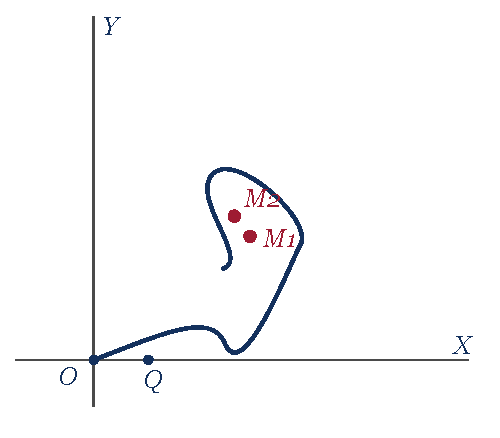
\includegraphics[width=0.55\textwidth]{figuras/pdf/cap04-fig5.pdf}
\caption{Puntos $M_1$, $M_2$ sobre la espiral, correspondientes a los
límites $v_1$, $v_2$ de la integral de Fresnel.}
\label{fig:cap4-5}
\end{figure}

Para que haya máximo o mínimo, es necesario que el triángulo formado por
la cuerda y las tangentes $M_1T$ y $M_2T$ (figura~\ref{fig:cap4-6}) sea
isósceles, o bien que las tangentes en los extremos sean paralelas y del
mismo sentido (figura~\ref{fig:cap4-7}). Tendremos así dos categorías de
máximos y de mínimos.

\begin{figure}[h]
\centering
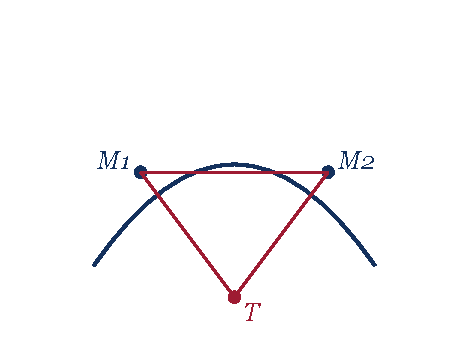
\includegraphics[width=0.55\textwidth]{figuras/pdf/cap04-fig6.pdf}
\caption{Triángulo isósceles formado por la cuerda $M_1M_2$ y las
tangentes que se cortan en $T$: primera categoría de extremos.}
\label{fig:cap4-6}
\end{figure}

\begin{figure}[h]
\centering
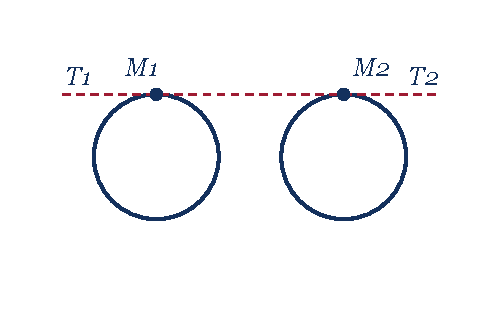
\includegraphics[width=0.7\textwidth]{figuras/pdf/cap04-fig7.pdf}
\caption{Tangentes paralelas y de igual sentido en $M_1$ y $M_2$: segunda
categoría de extremos.}
\label{fig:cap4-7}
\end{figure}

Para la segunda categoría deberá tenerse
\[
\frac{\pi}{2}v_2^2 = \frac{\pi}{2}v_1^2 + 2K\pi,
\]
siendo $\dfrac{\pi}{2}v^2$ el ángulo formado por la tangente en un punto
con el eje $x$. Esta igualdad nos da $v_2^2-v_1^2=4K$, o bien
\[
v_2+v_1 = \frac{4K}{l},
\]
poniendo $l=v_2-v_1$.

En cuanto a los máximos y mínimos de la primera categoría, su búsqueda es
muy complicada.

\section{Difracción por el borde de una pantalla}

\noindent\textbf{101. Difracción por el borde de una pantalla.} — En este
caso, el límite $v_2$ de la integral (3) del §96 es infinito y la
intensidad luminosa en un punto $P$ es proporcional al cuadrado del
módulo de
\[
\int_{v_1}^{\infty} e^{\frac{i\pi}{2}v^2}\,dv.
\]
Si $M_1$ es el punto correspondiente a $v_1$, este módulo es igual a la
longitud $AM_1$ de la recta que une el punto asintótico $A$ con el punto
$M_1$.

Cuando el punto $P$ está en el interior de la sombra geométrica, su polo
$Q$ está sobre la pantalla; por consiguiente, el límite inferior $v_1$ de
la integral precedente es positivo y el punto $M_1$ que le corresponde
está en la parte de la curva situada del mismo lado que $A$
(figura~\ref{fig:cap4-8}). La intensidad va, pues, decreciendo muy
rápidamente en cuanto nos alejamos del borde de la sombra geométrica sin
presentar ni máximo ni mínimo.

\begin{figure}[h]
\centering
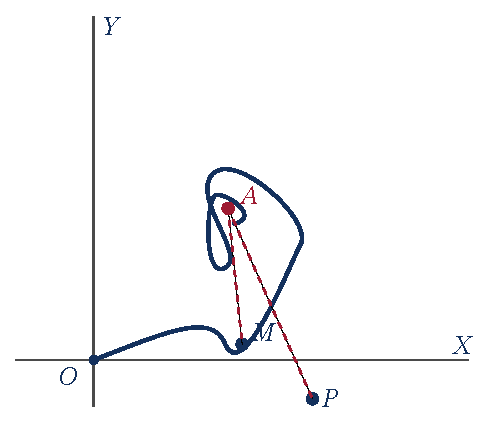
\includegraphics[width=0.6\textwidth]{figuras/pdf/cap04-fig8.pdf}
\caption{El punto asintótico $A$, el punto $M$ y la distancia $AM$ en la
sombra geométrica del borde de una pantalla.}
\label{fig:cap4-8}
\end{figure}

Siendo $AM$ aproximadamente igual a $\dfrac{1}{\pi v}$, el cuadrado del
módulo de nuestra integral es igual aproximadamente a $\dfrac{1}{\pi^2v^2}$.

Por consiguiente, del lado de la sombra geométrica, la intensidad
luminosa varía sensiblemente en razón inversa del cuadrado de la
distancia al borde de esa sombra.

Si el punto $P$ está fuera de la sombra geométrica, su polo $Q$ está
fuera de la pantalla; el valor límite $v_1$ es negativo y el punto $M_1$
está en la parte de la curva situada debajo del eje $x$. La recta $AM_1$
y, por consiguiente, la intensidad en $P$, presentarán una sucesión de
máximos y de mínimos; tendremos franjas. Los máximos y mínimos de $AM_1$
corresponden a los puntos donde esta recta es normal a la curva. Cuando
el punto $M_1$ es vecino de $A'$, las normales a la curva que pasan por
$A$ difieren poco de la recta $AA'$
(figura~\ref{fig:cap4-9}). Formando esta recta con $ox$ un ángulo igual a
$\dfrac{\pi}{4}$, la tangente en un punto correspondiente a un máximo o a
un mínimo forma con $ox$ un ángulo dado por la fórmula
\[
-\frac{\pi}{4}+K\pi.
\]

\begin{figure}[h]
\centering
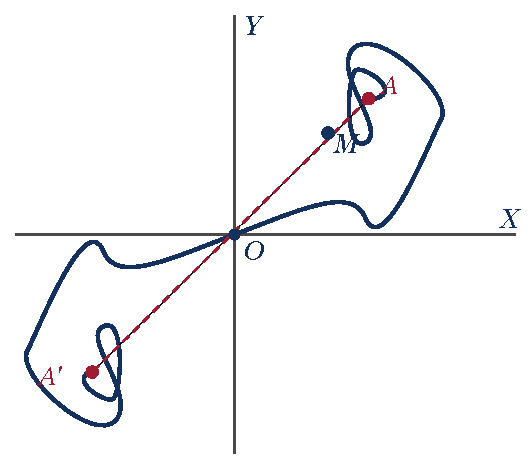
\includegraphics[width=0.6\textwidth]{figuras/pdf/cap04-fig9.pdf}
\caption{Los dos puntos asintóticos $A$, $A'$ y la recta $AA'$, que forma
un ángulo de $\pi/4$ con el eje $ox$.}
\label{fig:cap4-9}
\end{figure}

Teniendo este ángulo por valor, en función de $v$, $\dfrac{\pi}{2}v^2$,
tendremos la igualdad
\[
\frac{\pi}{2}v^2 = -\frac{\pi}{4}+K\pi,
\]
que nos dará, para $v^2$,
\[
v^2 = 2K-\frac12.
\]
Tal es la fórmula que da aproximadamente los valores de $v^2$
correspondientes a los máximos y mínimos.

Sean $M_1$ y $M_2$ dos puntos correspondientes a un máximo y a un mínimo
consecutivos. La diferencia de intensidad será
\[
AM_1^2 - AM_2^2.
\]
Si el máximo es de orden elevado, los puntos $M_1$ y $M_2$ estarán muy
próximos el uno del otro y estarán sensiblemente sobre la recta $AA'$;
tendremos entonces, sensiblemente,
\[
AM_1+AM_2 = 2AA',\qquad
AM_1-AM_2 = A'M_1+A'M_2 = \frac1{\pi v_1}+\frac1{\pi v_2},
\]
siendo $v_1$ y $v_2$ los valores de $v$ que corresponden a $M_1$ y a
$M_2$. La diferencia de intensidad será, pues,
\[
2AA'\left(\frac1{v_1}+\frac1{v_2}\right),
\]
lo que muestra que la diferencia entre un máximo y un mínimo consecutivos
varía sensiblemente en razón inversa de la distancia al borde de la
sombra geométrica.

\section{Difracción por una pequeña pantalla circular}

\noindent\textbf{102. Difracción por una pequeña pantalla circular.} —
Supongamos que una pequeña pantalla circular ocupa una parte de la esfera
$S$. Para obtener las variaciones de la intensidad luminosa en los
distintos puntos de un plano situado a una distancia $b$ del centro de la
pantalla, deberemos, como antes, estudiar las variaciones de la integral
\begin{equation}
\iint e^{\frac{i\pi}{2}(u^2+v^2)}\,du\,dv,
\tag{1}
\end{equation}
extendida a todos los puntos del plano tangente a la esfera en $Q$, que
están fuera de la pantalla.\footnote{A partir de aquí, y durante el resto
del capítulo, Poincaré reinicia la numeración de sus ecuaciones en casi
cada nueva subsección —ya ocurrió varias veces en la primera mitad del
capítulo—. Conservamos cada numeración tal como aparece en el original,
sin renumerar de forma continua.}

Busquemos en particular la iluminación en un punto situado sobre la recta
que une la fuente luminosa con el centro de la pantalla; el polo del
punto considerado se encuentra entonces en el centro de la pantalla.
Pongamos
\[
u=\rho\cos\varphi,\qquad v=\rho\sin\varphi.
\]
Tendremos
\[
\rho^2=u^2+v^2,
\]
y, como $u$ y $v$ son proporcionales a las distancias de un punto del
plano tangente en $Q$ a dos ejes rectangulares que pasan por $Q$, $\rho$
será proporcional a la distancia de ese punto a $Q$. Por consiguiente, si
tomamos como coordenadas $\rho$ y $\varphi$, los bordes de la pantalla
tendrán para $\rho$ un valor constante $a$. El producto $du\,dv$,
proporcional a la superficie de un elemento, se convierte en este sistema
de coordenadas en $\rho\,d\rho\,d\varphi$; por consiguiente, la integral
que da la intensidad es
\begin{equation}
\int_a^\infty\int_0^{2\pi} e^{\frac{i\pi}{2}\rho^2}\,\rho\,d\rho\,d\varphi.
\tag{2}
\end{equation}
Integrando respecto de $\varphi$, se tiene
\begin{equation}
2\pi\int_a^\infty e^{\frac{i\pi}{2}\rho^2}\,\rho\,d\rho;
\tag{3}
\end{equation}
y haciendo la integración respecto de $\rho$, se obtiene
\[
2\pi\left[\frac{1}{i\pi}e^{\frac{i\pi}{2}\rho^2}\right]_a^\infty
= -2i\left[e^{\frac{i\pi}{2}\rho^2}\right]_a^\infty.
\]
Para el límite $\rho=\infty$, el valor de la exponencial imaginaria es
indeterminado. Tomaremos para este valor cero, pues nuestras fórmulas
solo se aplican al caso en que $\rho$ es pequeño, y los elementos de la
integral (3) que corresponden a valores muy grandes de $\rho$ no deben
considerarse. Tendremos, pues, simplemente,
\[
\iint e^{\frac{i\pi}{2}(u^2+v^2)}\,du\,dv = 2i\,e^{\frac{i\pi}{2}a^2}.
\]
El módulo de esta última exponencial es 2. La intensidad luminosa en el
punto considerado es, pues, independiente de $a$, y por consiguiente del
radio de la pantalla; tiene el mismo valor que si $a=0$, es decir, que si
la pantalla no existiera.

Esta consecuencia de las fórmulas de difracción fue hallada por Poisson.
Fresnel verificó experimentalmente la presencia de este punto luminoso en
el centro de la sombra geométrica dada por una pequeña pantalla circular.

\begin{notahistorica}
Este es el célebre \emph{punto de Poisson} (también llamado punto de
Arago), ya mencionado en el Capítulo III a propósito de la controversia
entre Fresnel y Poisson sobre el principio de Huygens: una predicción que
Poisson creía absurda y que Arago confirmó experimentalmente, en una de
las demostraciones más contundentes de la naturaleza ondulatoria de la
luz.
\end{notahistorica}

Se concibe fácilmente que este fenómeno no se produzca sino con una
pequeña pantalla, pues, en caso contrario, nuestras fórmulas ya no son
aplicables. En efecto, hemos visto (§95) que la intensidad en un punto
depende de los valores de $\xi_1$ y de $\dfrac{d\xi_1}{dt}$ en los
distintos puntos de la esfera $S$, valores que hemos supuesto constantes;
lo cual no puede ser cierto sino si consideramos una porción muy pequeña
de la esfera $S$.

\section{Difracción por una pequeña abertura circular}

\noindent\textbf{103. Difracción por una pequeña abertura circular.} —
En este caso, los límites de la integral (3) del párrafo precedente son
$0$ y $a$. Tenemos, pues, para la intensidad en un punto cuyo polo ocupa
el centro de la abertura, una cantidad proporcional al módulo de
\[
2i\left(1-e^{\frac{i\pi}{2}a^2}\right).
\]
El módulo del primer factor es 2, el del segundo factor varía de 0 a 2
con el valor de $a$. Este módulo es nulo para $a^2=4K$, siendo $K$ un
entero; es igual a 2 para $a^2=4K+2$. Tendremos, pues, en un mismo punto
del espacio, oscuridad o luz según el radio de la abertura. Alrededor de
ese punto, se tendrán franjas que, por razón de simetría, deberán ser
circulares.

\section{Difracción en luz paralela}

\noindent\textbf{104. Difracción en luz paralela.} — Un caso
particularmente interesante de la difracción es aquel en que se observan
los fenómenos a gran distancia de una pantalla colocada muy lejos de la
fuente luminosa. Podremos entonces considerar el radio de la esfera que
contiene la pantalla como infinito, y esta esfera se convertirá en un
plano.

Sea $P$ (figura~\ref{fig:cap4-10}) un punto del espacio; una de las
componentes del desplazamiento de este punto será la parte real de
\[
\xi = e^{-i\alpha Vt}\int X\,\frac{e^{i\alpha r}}{r}\,d\omega,
\]
siendo $X$ una función del desplazamiento $\xi_1$ de un punto del plano
$R$, y extendiéndose la integral a todos los puntos de ese plano.

\begin{figure}[h]
\centering
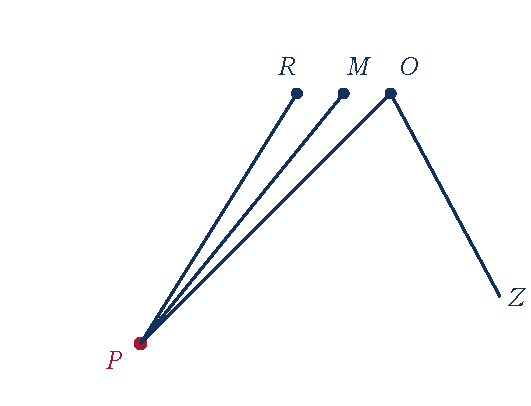
\includegraphics[width=0.75\textwidth]{figuras/pdf/cap04-fig10.pdf}
\caption{Difracción en luz paralela: el punto $P$, el plano $R$ con los
puntos $M$ y $O$ vecinos, y la dirección $OZ$.}
\label{fig:cap4-10}
\end{figure}

Hemos visto que cuando la pantalla no estaba muy alejada de la fuente
luminosa, solo la porción de la esfera vecina del polo del punto $P$
tenía influencia sobre la iluminación de ese punto. Lo mismo ocurrirá
cuando el radio de la esfera se vuelva infinito, y no tendremos que
considerar en la búsqueda de la iluminación del punto $P$ más que los
puntos del plano $R$ vecinos del pie de la perpendicular bajada de $P$
sobre el plano. Podremos, pues, suponer que la función $X$ tiene un valor
constante y sacarla del signo de integración. Además, estando el punto
$P$ supuesto alejado del plano, sus distancias $PO$ y $PM$ a dos puntos
vecinos $M$ y $O$ diferirán poco la una de la otra, y podremos considerar
el factor $\dfrac1r$ como teniendo el mismo valor para todos los
elementos de la integral que no son despreciables. Tendremos, pues, para
esta integral
\[
\int X\,\frac{e^{i\alpha r}}{r}\,d\omega = \frac{X}{r}\int e^{i\alpha r}\,d\omega
= \frac{X e^{i\alpha r_0}}{r}\int e^{i\alpha(r-r_0)}\,d\omega,
\]
llamando $r_0$ a la distancia del punto $P$ a un punto arbitrario $O$ del
plano $Q$.

\noindent\textbf{105.} Por las mismas consideraciones que las expuestas
en el §95, llegaríamos a mostrar que la intensidad luminosa de los
distintos puntos de un plano paralelo a $R$ es proporcional al cuadrado
del módulo de la integral
\begin{equation}
\int e^{i\alpha(r-r_0)}\,d\omega.
\tag{1}
\end{equation}
Transformemos esta integral. Desde el punto $M$ bajemos sobre $OP$ la
perpendicular $MM'$ y designemos por $P$ el ángulo $OPM$ y por $r$ la
distancia $PM$; tendremos
\[
PM' = r\cos P = r - r(1-\cos P) = r - 2r\sin^2\frac{P}{2}.
\]
El ángulo $P$ es muy pequeño, puesto que solo consideramos puntos del
plano $R$ vecinos los unos de los otros; por consiguiente $\sin^2\dfrac{P}{2}$
es el cuadrado de una cantidad muy pequeña, y aunque $r$ se suponga muy
grande, el producto $2r\sin^2\dfrac{P}{2}$ será despreciable. Tendremos
$PM'=r$ y $OM'=r_0-r$.

Tomemos en el plano $R$ dos ejes de coordenadas rectangulares que pasen
por $O$. Si designamos por $x$ e $y$ las coordenadas de $M$ y por $l$ y
$m$ los cosenos de la dirección $OP$ con los ejes, tendremos para $OM'$,
que es la proyección de $OM$ sobre $OP$,
\[
OM' = lx+my,
\]
y por consiguiente,
\[
r_0-r = lx+my.
\]
Llevando esta expresión de $r_0-r$ a la integral (1), se convierte en
\[
\int e^{-i\alpha(lx+my)}\,d\omega;
\]
pero, como solo tenemos que considerar el cuadrado del módulo de esta
integral, podemos tomar
\begin{equation}
\int e^{i\alpha(lx+my)}\,d\omega,
\tag{2}
\end{equation}
cuyo módulo es el mismo.

\section{Franjas producidas por una abertura con centro de simetría}

\noindent\textbf{106. Franjas producidas por una abertura con centro de
simetría.} — En general los mínimos de intensidad luminosa no son nulos,
pues el módulo de nuestra integral solo podría anularse si la parte real
y la parte imaginaria se anularan a la vez, lo que en general no ocurrirá;
pero en el caso de la difracción producida por una abertura que tiene un
centro de simetría, esos mínimos son iguales a cero.

En efecto, si suponemos que el punto $O$ es el centro de simetría de la
abertura, la integral
\[
\int e^{i\alpha(lx+my)}\,d\omega,
\]
extendida a todos los puntos de la abertura, debe conservar el mismo
valor cuando se cambia $x$ en $-x$ e $y$ en $-y$. Con este cambio la
integral se convierte en
\[
\int e^{-i\alpha(lx+my)}\,d\omega.
\]
La parte imaginaria de esta integral es de signo contrario a la parte
imaginaria de la integral precedente. Como estas dos integrales tienen el
mismo valor, la parte imaginaria es nula y cada una de ellas se reduce a
la parte real,
\[
\int \cos\alpha(lx+my)\,d\omega.
\]
Esta integral es real y no es en general siempre del mismo signo, de modo
que debe anularse; por lo tanto, en luz homogénea los mínimos de
intensidad son rigurosamente nulos.

\section{Difracción por aberturas semejantes}

\noindent\textbf{107. Difracción por aberturas semejantes.} — Designemos
por $\delta$ el ángulo de la dirección $OP$ (figura~\ref{fig:cap4-10}) con
la perpendicular en $O$ al plano de la abertura. Vamos a mostrar que si
reemplazamos esta abertura por una abertura semejante cuya razón de
similitud con la primera es $K$, el seno del ángulo de desviación
$\delta$ que corresponde a una misma franja queda dividido por $K$.

Si $x$ e $y$ son las coordenadas de un punto de la primera abertura, las
coordenadas del punto correspondiente en la abertura semejante serán
$Kx$ y $Ky$. La intensidad luminosa en un punto $P$ al que corresponden
los cosenos directores $l$ y $m$ será, en el caso de la primera abertura,
proporcional al cuadrado del módulo de
\[
\int e^{i\alpha(lx+my)}\,d\omega,
\]
y en el caso de la segunda, al cuadrado del módulo de
\[
\int e^{i\alpha K(lx+my)}\,K^2\,d\omega.
\]
Si consideramos un punto $P_1$ situado siempre a la misma distancia del
plano $R$, pero cuyos cosenos con los ejes $x$ e $y$ son $\dfrac{l}{K}$ y
$\dfrac{m}{K}$, la intensidad luminosa en ese punto será, con la segunda
abertura, proporcional al cuadrado del módulo de
\[
\int e^{i\alpha(lx+my)}\,K^2\,d\omega.
\]
Esta intensidad será proporcional a la intensidad en el punto $P$
supuesto iluminado por la rendija primitiva, y los máximos o mínimos de
estas intensidades tendrán lugar al mismo tiempo. Busquemos el seno del
ángulo de desviación $\delta_1$ del punto $P_1$. Llamando $\varphi$ al
ángulo del plano $POZ$ con el plano de los $xz$, se tiene
\[
l=\sin\delta\cos\varphi\qquad m=\sin\delta\sin\varphi.
\]
Por consiguiente
\[
\sin^2\delta = l^2+m^2.
\]
Para el punto $P_1$ tendremos
\[
\sin^2\delta_1 = \frac{l^2}{K^2}+\frac{m^2}{K^2},
\]
y por consiguiente
\[
\sin^2\delta_1 = \frac{\sin^2\delta}{K^2}.
\]

Esta igualdad nos muestra que si se reemplaza una abertura por una
segunda $K$ veces más grande, el seno del ángulo de desviación
correspondiente a una misma franja queda dividido por $K$; el plano de
difracción será, por lo demás, el mismo, puesto que la razón $\dfrac{l}{m}$
no ha variado.

Así, dos aberturas semejantes producirán figuras de difracción
semejantes; pero las dimensiones de estas figuras estarán en razón
inversa de las dimensiones de las aberturas.

\section{Teorema de Bridge}

\noindent\textbf{108. Teorema de Bridge.} —

\begin{enunciado}{Teorema de Bridge}
Cuando una pantalla está perforada por varias aberturas idénticas y
dispuestas de manera semejante, la intensidad en un punto es igual a la
intensidad resultante de una sola abertura multiplicada por la intensidad
debida a un conjunto de puntos luminosos dispuestos en el plano como lo
están las aberturas.
\end{enunciado}

La intensidad en un punto $P$ es proporcional al cuadrado del módulo de
la integral
\begin{equation}
\int e^{i\alpha(lx+my)}\,d\omega,
\tag{1}
\end{equation}
extendida a todas las porciones iluminadas de la pantalla. Esta integral
será la suma de integrales de la misma forma extendidas a la superficie
de cada una de las aberturas. Siendo estas aberturas iguales y dispuestas
de manera semejante, si a un punto de coordenadas $x$ e $y$ de una de
ellas corresponde un punto de coordenadas $x+a$ e $y+b$ de otra,
tendremos todos los puntos de esta última dando a $x$ e $y$ todos los
valores que estas cantidades pueden tomar en la primera abertura. Por
consiguiente, el término de la integral (1) que corresponde a una
abertura cualquiera es igual a
\[
\int e^{i\alpha(l(a+x)+m(b+y))}\,d\omega
= e^{i\alpha(la+mb)}\int e^{i\alpha(lx+my)}\,d\omega,
\]
estando estas integrales extendidas a toda la superficie de una de las
aberturas. La integral (1) tendrá, pues, por valor el producto
\[
\left(1+e^{i\alpha(la+mb)}+\ldots\right)\int e^{i\alpha(lx+my)}\,d\omega,
\]
que se puede escribir
\[
\sum e^{i\alpha(la+mb)}\int e^{i\alpha(lx+my)}\,d\omega,
\]
obteniéndose la unidad al hacer $a=b=0$.

El cuadrado del módulo del primer factor es proporcional a la intensidad
luminosa debida a $n$ puntos dispuestos en el plano como lo están las
aberturas de la pantalla; el cuadrado del módulo de la integral es
proporcional a la intensidad debida a una sola abertura. El teorema de
Bridge queda, pues, demostrado.

\section{Teorema de Babinet}

\noindent\textbf{109. Teorema de Babinet.} —

\begin{enunciado}{Teorema de Babinet}
Dos pantallas complementarias, es decir, tales que a los vacíos de una
corresponden los llenos de la otra, dan en un punto del espacio la misma
iluminación, excepto si ese punto está en la dirección de $oz$.
\end{enunciado}

\begin{notahistorica}
Jacques Babinet (1794-1872), físico y astrónomo francés, enunció este
principio en 1837. Es un resultado notable porque permite deducir
inmediatamente el patrón de difracción de una pantalla a partir del de su
complementaria —por ejemplo, el de un disco opaco a partir del de una
abertura circular del mismo tamaño— sin necesidad de un nuevo cálculo.
\end{notahistorica}

Designemos por $R$ la porción iluminada de la primera pantalla y por $R'$
la porción iluminada de la segunda. Como a las partes no iluminadas de la
primera pantalla corresponden las partes iluminadas de la segunda, la
suma de las superficies $R$ y $R'$ debe ser igual a todo el plano. La
intensidad luminosa en un punto del espacio será, con la primera
pantalla, proporcional al cuadrado del módulo de la integral
\[
\int e^{i\alpha(lx+my)}\,d\omega.
\]
extendida a toda la porción iluminada de la pantalla. Con la segunda
pantalla, será preciso, para obtener la intensidad, extender esta
integral a todos los puntos de la porción iluminada $R'$ de la pantalla.
La suma de estas dos integrales será la integral extendida a todo el
plano, es decir,
\[
\int_{-\infty}^{+\infty} e^{i\alpha(lx+my)}\,d\omega.
\]

El cuadrado del módulo de esta integral representa la iluminación debida
a una abertura muy grande; según lo que hemos visto a propósito de las
aberturas semejantes, los ángulos de desviación son tanto más pequeños
cuanto mayores son las dimensiones de la abertura. Para una abertura muy
grande, las desviaciones serán muy pequeñas, es decir, que no habrá luz
sensible más que en la dirección del eje de las $z$.

Esta integral es, pues, nula para todos los puntos del espacio que no son
vecinos del eje $oz$. Por consiguiente, para todos esos puntos, las
integrales que sirven para hallar la intensidad en un punto no
diferirán más que por el signo y el cuadrado de su módulo tendrá el mismo
valor. La intensidad luminosa es, pues, la misma en esos puntos.

\section{Difracción por aberturas alargadas}

\noindent\textbf{110. Difracción por aberturas alargadas.} — Supongamos
que reemplazamos la abertura de una pantalla por otra obtenida
multiplicando las ordenadas de cada punto de la primera por la misma
cantidad $K$ sin cambiar las abscisas. En tal transformación un cuadrado
se convierte en un rectángulo, un círculo se convierte en una elipse.

La intensidad luminosa en un punto del espacio cuando se toma la segunda
abertura es proporcional al cuadrado del módulo de la integral
\[
\int e^{i\alpha(lx+Kmy)}\,K\,d\omega.
\]
Por consiguiente, la intensidad luminosa dada por la segunda abertura en
un punto $P_1$ al que corresponden los cosenos $l$ y $\dfrac{m}{K}$ será
$K$ veces la intensidad dada por la primera abertura en un punto $P$ tal
que los cosenos directores de $OP$ sean $l$ y $m$.

Si en el plano que pasa por $P$ y es paralelo al plano $R$ de la
figura~\ref{fig:cap4-10}, trazamos ejes de coordenadas paralelos a los
$x$ y a los $y$ trazados en el plano $R$, las coordenadas $x_1$ e $y_1$
de $P$ respecto de estos ejes serán iguales a las coordenadas de la
proyección de ese punto sobre el plano $R$. Los cosenos directores de la
dirección $OP$ son $l$, $m$ y $\cos\delta$; por consiguiente, designando
por $z$ la distancia constante del punto $P$ al plano $R$, se tiene
\[
x_1 = \frac{lz}{\cos\delta}\qquad y_1 = \frac{mz}{\cos\delta},
\]
o, reemplazando $\cos\delta$ por su valor en función de $l$ y de $m$,
\[
x_1 = \frac{lz}{\sqrt{1-l^2-m^2}}\qquad y_1 = \frac{mz}{\sqrt{1-l^2-m^2}}.
\]

Por consiguiente, cuando se reemplaza una abertura por otra cuyas
ordenadas son $K$ veces más grandes, las coordenadas del punto cuya
intensidad es $K$ veces la que poseía el punto $x_1$, $y_1$ con la
abertura primitiva son
\[
x_1' = \frac{lz}{\sqrt{1-l^2-\dfrac{m^2}{K^2}}}\qquad
y_1' = \frac{mz}{K\sqrt{1-l^2-\dfrac{m^2}{K^2}}}.
\]
Este punto se ha, pues, acercado al eje de las $x_1$.

Las desviaciones son generalmente pequeñas, de modo que podemos
despreciar $l^2$ y $m^2$ y escribir
\[
x_1=lz,\qquad y_1=mz,\qquad x_1'=lz,\qquad y_1'=\frac{mz}{K},
\]
o bien
\[
x_1=x_1',\qquad y_1'=\frac{y_1}{K}.
\]
La abscisa del punto que corresponde a un máximo de intensidad no ha
cambiado, pues, mientras que la ordenada se ha vuelto $K$ veces más
pequeña. Se deducirán, pues, las nuevas figuras de difracción de las
antiguas multiplicando las ordenadas de todos los puntos por
$\dfrac{1}{K}$.

Supongamos en particular que la abertura primitiva sea circular. Por
razón de simetría, las franjas de difracción serán también circulares.
Si multiplicamos las ordenadas de los distintos puntos de la abertura por
$K$, esta abertura se convertirá en una elipse. Para obtener las nuevas
franjas de difracción, será necesario multiplicar las ordenadas de las
antiguas franjas por $\dfrac1K$; estas franjas se convertirán así en
elípticas.

Así, una abertura elíptica produce figuras de difracción que son también
elipses. Estas elipses son semejantes a la abertura pero inversamente
colocadas, siendo el eje mayor de las franjas elípticas paralelo al eje
menor de la abertura.

Si tomamos una rendija muy alargada, los puntos donde la intensidad es
nula estarán muy cerca del eje de las $x_1$, pues se puede considerar tal
rendija como resultante de un cuadrado cuyo lado paralelo al eje de las
$y$ se ha multiplicado por un número muy grande $K$. No se observarán,
pues, los fenómenos de difracción más que en el plano de los $xz$, es
decir, en un plano perpendicular a la longitud de la rendija.

\section{Difracción por una rendija o pantalla rectangular}

\noindent\textbf{111. Difracción por una rendija o pantalla rectangular.}
— Designemos por $2a$ y $2b$ las dimensiones de la rendija. Para obtener
la intensidad luminosa dada en un punto $P$ por esta abertura, debemos
considerar la integral
\[
\int e^{i\alpha(lx+my)}\,d\omega,
\]
extendida a toda la superficie de la rendija. El elemento de superficie
$d\omega$ siendo igual al producto $dx\,dy$, tendremos para nueva forma
de esta integral
\[
\iint e^{i\alpha(lx+my)}\,dx\,dy;
\]
y como podemos suponer que el origen de las coordenadas coincide con el
centro de la rendija, los límites de integración serán $-a$ y $+a$ para
$x$, y $-b$ y $+b$ para $y$. Siendo constantes los límites de
integración, la integral precedente es el producto de las dos integrales
simples, tomadas una respecto de $x$, y la otra respecto de $y$.
Tendremos que buscar el módulo del producto
\[
\int_{-a}^{+a} e^{i\alpha lx}\,dx \int_{-b}^{+b} e^{i\alpha my}\,dy.
\]
Para simplificar nuestras expresiones, pongamos
\begin{equation}
\alpha l=u\qquad \alpha m=v;
\tag{1}
\end{equation}
tendremos
\[
\int_{-a}^{+a} e^{iux}\,dx \int_{-b}^{+b} e^{ivy}\,dy.
\]
La primera integral de este producto tiene por valor
\[
\frac{e^{iau}-e^{-iau}}{iu} = \frac{2\sin au}{u}.
\]
El valor de la integral tomada respecto de $y$ es
\[
\frac{e^{ibv}-e^{-ibv}}{iv} = \frac{2\sin bv}{v}.
\]
El producto de las dos integrales será
\[
4\,\frac{\sin au}{u}\cdot\frac{\sin bv}{v},
\]
o también
\[
4ab\,\frac{\sin au}{au}\cdot\frac{\sin bv}{bv}.
\]
Tendremos, pues, para la intensidad luminosa, una cantidad proporcional a
\begin{equation}
\left(\frac{\sin au}{au}\right)^2 \times \left(\frac{\sin bv}{bv}\right)^2.
\tag{2}
\end{equation}
Esta intensidad se volverá nula cuando uno de los senos sea nulo, es
decir, para
\begin{equation}
au=K\pi,\qquad\text{o}\qquad bv=K'\pi,
\tag{3}
\end{equation}
donde $K$ y $K'$ son enteros cualesquiera, pero que no pueden suponerse
nulos. En efecto, para $K=0$ o $K'=0$, el valor de los dos factores
$\dfrac{\sin au}{au}$, $\dfrac{\sin bv}{bv}$ es la unidad, y por
consiguiente la intensidad no es nula; es incluso máxima, siendo la
unidad el mayor valor absoluto que puede tomar cada uno de los factores.
Observemos que si $K$ y $K'$ son nulos se tiene $u=v=0$ y por
consiguiente $l=m=0$. El punto cuya iluminación se busca está entonces
situado sobre el eje $oz$ (figura~\ref{fig:cap4-10}), es decir, sobre una
perpendicular al plano de la rendija elevada por el centro de esta
rendija. En todo punto de esta recta la intensidad es máxima.

\noindent\textbf{112.} Los valores de $l$ y de $m$ que corresponden a los
mínimos de intensidad se obtienen reemplazando en las ecuaciones de
condición (3) $u$ y $v$ por sus valores (1); estos valores son
\[
l=\frac{K\pi}{a\alpha},\qquad m=\frac{K'\pi}{b\alpha}.
\]
Hemos visto (§110) que si se toman en el plano donde se observan los
fenómenos dos ejes paralelos a los ejes $x$ y $y$ y que se cortan sobre
$oz$, las coordenadas $x_1$ e $y_1$ de un punto son proporcionales a $l$ y
a $m$. Por consiguiente, los puntos cuya intensidad es nula están
situados sobre rectas paralelas a uno de los ejes de coordenadas y
equidistantes entre sí. El fenómeno tendrá, pues, el aspecto de una serie
de mallas rectangulares luminosas, cuyo centro presenta un máximo de
iluminación. Estos máximos decrecen muy rápidamente en cuanto nos
alejamos de los ejes, es decir, en cuanto $u$ o $v$ aumenta, puesto que
la expresión (2) a la cual es proporcional la intensidad contiene en el
denominador el producto $u^2v^2$. Así, apenas se ve más que una cruz
luminosa en la dirección de los ejes, formada por los puntos que
corresponden a $K=0$ o $K'=0$.

El teorema de Babinet nos indica que se tendrá el mismo fenómeno tomando
una pequeña pantalla rectangular.

Si una de las dimensiones de la rendija tiene un tamaño considerable, no
se tendrán, según el §110, fenómenos observables más que en el plano
perpendicular a la mayor dimensión de la rendija. Se verá una serie de
bandas de intensidad nula separadas por bandas luminosas cuyo brillo
decrece muy rápidamente a partir de la banda central. El cálculo muestra
que al segundo máximo corresponde una intensidad 20 veces menor que al
primero.

Los mismos fenómenos se observarían con un hilo.

\section{Caso de \texorpdfstring{$n$}{n} puntos luminosos irregularmente
dispuestos en un plano}

\noindent\textbf{113. Caso de $n$ puntos luminosos irregularmente
dispuestos en un plano.} — Llamando $a$ y $b$ a las coordenadas de uno
cualquiera de estos puntos, que supondremos de la misma intensidad, la
intensidad luminosa en un punto del espacio es proporcional al cuadrado
del módulo de la suma
\[
\sum e^{i(ua+vb)};
\]
ahora bien, el producto de dos cantidades imaginarias conjugadas es igual
al cuadrado del módulo de una de esas imaginarias; la intensidad luminosa
será, pues, proporcional a
\[
\sum e^{i(ua+vb)} \sum e^{-i(ua+vb)} = \sum e^{i[u(a-a')+v(b-b')]},
\]
siendo $a'$ y $b'$ las coordenadas de un segundo punto luminoso
cualquiera.

El número de términos de este producto es $n^2$. Para $n$ de entre ellos,
se tiene $a=a'$, $b=b'$ y el valor de cada uno de ellos es 1; su suma
será $n$. Para los $n^2-n$ términos restantes el módulo es 1 y el
argumento $u(a-a')+v(b-b')$. Este argumento puede tomar todos los valores
posibles puesto que los puntos están distribuidos irregularmente. Ahora
bien, se sabe que el valor medio de $e^{i\varphi}$, donde $\varphi$ puede
tomar todos los valores posibles, es cero; por consiguiente, la suma de
los $n^2-n$ términos considerados es nula. La intensidad en un punto
iluminado por los $n$ puntos de igual intensidad será, pues, una
constante igual a $n$ veces la intensidad dada por un solo punto
iluminante.

\section{Caso de \texorpdfstring{$n$}{n} aberturas}

\noindent\textbf{114. Caso de $n$ aberturas.} — Consideremos $n$ aberturas
iguales, dispuestas de manera semejante pero colocadas irregularmente en
el plano. Según el teorema de Bridge (§108), la intensidad será el
producto de dos factores, uno proporcional a la intensidad dada por una
sola rendija, y el otro proporcional a la intensidad dada por $n$ puntos
colocados en el plano como lo están las aberturas. Cuando estas aberturas
estén dispuestas irregularmente, este segundo factor será, según el
párrafo precedente, igual a $n$ veces la intensidad resultante de una
sola abertura.

El teorema de Babinet nos enseña que ocurriría lo mismo con $n$ pantallas.
En particular con $n$ pequeñas pantallas circulares se deberán tener los
mismos fenómenos que con una sola pantalla; los máximos de la intensidad
luminosa serán solamente $n$ veces más grandes. Se puede verificar este
hecho experimentalmente espolvoreando de licopodio el objetivo de un
anteojo astronómico; se perciben franjas negras y brillantes cuando se
hace la experiencia en luz homogénea.

\section{Caso de dos puntos de igual intensidad}

\noindent\textbf{115. Caso de dos puntos de igual intensidad.} — Tomemos
por eje de las $x$ una recta que pase por estos puntos, y por eje de las
$y$ una perpendicular trazada por el medio de la distancia que separa los
dos puntos. Las coordenadas de uno de los puntos serán $a$ y $0$, las del
otro, $-a$ y $0$. La intensidad luminosa en un punto del espacio será
proporcional al cuadrado del módulo de
\[
e^{iau}-e^{-iau}.
\]
Siendo esta diferencia igual a $2\cos au$,\footnote{Así en el original.
Debe leerse $e^{iau}+e^{-iau}$, que es la suma que corresponde a dos
puntos de igual intensidad y vale $2\cos au$; la diferencia escrita
valdría $2i\sin au$.} la intensidad es proporcional
a $\cos^2 au$. Los mínimos de intensidad tendrán lugar para
\[
u = \frac{(2K+1)\pi}{2a};
\]
estarán regularmente espaciados y su valor será nulo. Son debidos a la
interferencia de los rayos. Los máximos estarán regularmente espaciados e
iguales entre sí; corresponden a
\[
u = \frac{K\pi}{a}.
\]

\section{Caso de dos aberturas o de dos pantallas circulares}

\noindent\textbf{116. Caso de dos aberturas o de dos pantallas
circulares.} — Designando por $I$ la intensidad luminosa en un punto
cuando se tiene una sola abertura, y por $2a$ la distancia de los centros
de las dos aberturas, la intensidad dada por las dos aberturas será
proporcional a
\[
I\cos^2 au.
\]
Las variaciones del primer factor determinarán un sistema de franjas
concéntricas; las variaciones del segundo darán lugar a franjas
rectilíneas.

\section{Caso de dos rendijas rectangulares}

\noindent\textbf{117. Caso de dos rendijas rectangulares.} — Según el
§111, la intensidad resultante de una rendija de ancho $2b$ y cuya altura
es relativamente grande es proporcional a
\[
\left(\frac{\sin bu}{bu}\right)^2.
\]
Por consiguiente, para dos rendijas iguales distantes $2a$, tendremos
\[
\left(\frac{\sin bu}{bu}\right)^2 \cos^2 au.
\]
Los mínimos de intensidad, que serán nulos, tendrán lugar para
\[
u=\frac{K\pi}{b},\qquad u=\frac{(2K+1)\pi}{2a}.
\]
A los valores de $u$ dados por la primera igualdad corresponden franjas
de difracción, a los valores dados por la segunda corresponden franjas de
interferencia. Como $a$ es mayor que $b$, las franjas de interferencia
están más próximas entre sí que las franjas de difracción, y entre dos de
estas últimas siempre se encontrará cierto número de las primeras.

\section{Caso de \texorpdfstring{$n$}{n} puntos en línea recta y
equidistantes}

\noindent\textbf{118. Caso de $n$ puntos en línea recta y equidistantes.}
— Designemos por $2a$ la distancia de dos puntos consecutivos; tomemos
por eje de las $x$ la recta que pasa por todos los puntos y por origen el
primero de los puntos. Las abscisas serán
\[
0,\quad 2a,\quad 4a,\quad\ldots,\quad 2(n-1)a,
\]
y la integral cuyo cuadrado del módulo es proporcional a la intensidad se
convertirá en
\begin{equation}
1+e^{2iau}+e^{4iau}+\cdots+e^{2(n-1)iau}.
\tag{1}
\end{equation}
Los términos de esta suma forman una progresión geométrica cuya razón es
$e^{2iau}$; el valor de esta suma es, pues,
\[
\frac{e^{2niau}-1}{e^{2iau}-1}.
\]
No cambiaremos el módulo de esta fracción si la multiplicamos o la
dividimos por cantidades cuyo módulo es la unidad. Multipliquemos el
numerador por $e^{-niau}$ y el denominador por $e^{-iau}$; obtendremos
\[
\frac{e^{niau}-e^{-niau}}{e^{iau}-e^{-iau}},
\]
expresión que se puede escribir
\[
\frac{\sin nau}{\sin au}.
\]
La intensidad en un punto será proporcional al cuadrado de esta cantidad:
\begin{equation}
\frac{\sin^2 nau}{\sin^2 au}.
\tag{2}
\end{equation}

Estudiemos esta función. Es periódica, pues si aumentamos $u$ en
$\dfrac{\pi}{a}$, $au$ aumenta en $\pi$ y $nau$ en $n\pi$; por lo tanto el
valor absoluto de los senos no cambia.

Para los valores de $u$ dados por
\[
u=\frac{K\pi}{na},
\]
el numerador se anula y la función misma se vuelve nula, a menos que el
denominador no se anule al mismo tiempo que el numerador, lo que ocurre
para los valores de $K$ que son múltiplos de $n$. Para obtener el valor
que toma la función para los valores de $K$ múltiplos de $n$, nos basta,
puesto que la función es periódica, buscar qué se vuelve cuando se hace
$K=0$; se tiene en este caso
\[
\frac{\sin^2 nau}{\sin^2 au} = \frac{n^2a^2u^2}{a^2u^2} = n^2.
\]
La intensidad es proporcional a $n^2$; es un máximo absoluto de esta
intensidad, pues cada término de la suma (1) teniendo por módulo una
cantidad a lo sumo igual a 1, el módulo de la suma es a lo sumo igual a
$n$ y por consiguiente la intensidad tiene por valor máximo una cantidad
proporcional a $n^2$. Llamaremos máximos principales a los que
corresponden a una intensidad proporcional a $n^2$.

Entre dos de estos máximos la función (2) se anula $n-1$ veces, y entre
dos ceros consecutivos pasa por un máximo al menos; tendremos, pues, al
menos $n-2$ máximos secundarios. No puede además haber más, pues la
función es un polinomio entero de grado $n-1$ en $\cos au$; su derivada
respecto de $\cos au$ será de grado $n-2$ y no tendrá más que $n-2$
raíces, a cada una de las cuales corresponde un máximo o un mínimo.

Los máximos secundarios son muy pequeños y tanto menos aparentes cuanto
mayor es $n$. En efecto, se tiene
\[
\frac{\sin^2 nau}{\sin^2 au} < \frac{1}{\sin^2 au}.
\]
Si $\sin au$ tiene un valor finito, el segundo miembro de la desigualdad,
y por consiguiente el primero, son muy pequeños respecto de $n^2$.

Cuando $\sin au$ es pequeño, es decir, para los valores de $u$ vecinos de
$\dfrac{K\pi}{a}$, los máximos secundarios que están entonces vecinos de
los máximos principales son todavía difícilmente observables. En este
caso, estando $au$ vecino de $K\pi$, podemos, a causa de la periodicidad
de la función, suponer $au$ muy poco diferente de cero, y reemplazar
$\sin au$ por el arco; tendremos para el factor de intensidad
\[
\frac{\sin^2 nau}{a^2u^2}.
\]
El cálculo de este factor mostraría que el primer máximo secundario es 20
veces más pequeño que el máximo principal y el segundo, 60 veces más
pequeño.

\section{Redes de difracción}

\noindent\textbf{119. Redes.} — En una red tenemos $n$ rendijas de igual
ancho $2b$, paralelas y colocadas a una distancia $2a$ unas de otras. El
factor de intensidad de una sola rendija siendo
\begin{equation}
\frac{\sin^2 bu}{b^2u^2},
\tag{1}
\end{equation}
el de $n$ puntos equidistantes,
\begin{equation}
\frac{\sin^2 nau}{\sin^2 au},
\tag{2}
\end{equation}
la intensidad dada por la red será proporcional al producto de estos dos
factores. Como las rendijas tienen una altura grande respecto de su
ancho, solo se observarán franjas en un plano perpendicular a la longitud
de las rendijas.

Deberíamos, pues, observar los máximos debidos a los dos factores, pero
como $n$ es generalmente muy grande, solo serán visibles los máximos
principales debidos al factor (2). Para estos máximos, se tiene
\[
u=\frac{K\pi}{a},
\]
y la intensidad es proporcional a
\begin{equation}
n^2\,\dfrac{\sin^2\dfrac{Kb\pi}{a}}{\dfrac{K^2\pi^2b^2}{a^2}}.
\tag{3}
\end{equation}
Esta cantidad, conteniendo $K^2$ en el denominador, los máximos
principales disminuirán de intensidad a medida que nos alejemos de la
normal al plano de la red.

Si $\dfrac{b}{a}$ es muy pequeño, el producto $K\dfrac{b}{a}$ será menor
que $\dfrac12$ para un gran número de valores de $K$. En este caso el
numerador de (3) irá constantemente decreciendo y, como no se pueden
observar más de 6 o 7 máximos principales, irán decreciendo de
intensidad.

Cuando $\dfrac{b}{a}$ no es muy pequeño, el producto $K\dfrac{b}{a}$
puede volverse mayor que $\dfrac12$ para valores de $K$ inferiores a 7, y
entonces los máximos principales no decrecen regularmente, oscilando el
numerador de (3) entre 0 y 1.

Si el cociente $\dfrac{b}{a}$ es conmensurable, existe un valor de $K$
que anula $\sin\dfrac{Kb\pi}{a}$; por consiguiente, faltará el máximo
principal correspondiente. Así, si $\dfrac{b}{a}=\dfrac12$, faltarán
todos los máximos principales de orden par. En este caso particular,
$\sin\dfrac{Kb\pi}{a}$ tiene por valor absoluto la unidad cuando $K$ es un
número impar. Los máximos principales de orden impar serán
proporcionales a $\dfrac{1}{K^2}$; irán decreciendo regularmente.

Observemos que el intervalo lleno que separa dos rendijas es igual a
$2a-2b$; si, pues, cambiamos $2b$ en $2a-2b$, es decir, $b$ en $a-b$, en
nuestras fórmulas de intensidad, tendremos la intensidad resultante de
una nueva red que no difiere de la primera sino en que los espacios
opacos reemplazan a las rendijas y recíprocamente. Cambiando $b$ en
$a-b$ en $\sin\dfrac{Kb\pi}{a}$, obtenemos
\[
\sin\frac{K(a-b)\pi}{a} = \sin\left(K\pi-\frac{Kb\pi}{a}\right)
= \pm\sin\frac{Kb\pi}{a}.
\]
Por consiguiente, la fórmula (3) se convierte en
\[
n^2\,\dfrac{\sin^2\dfrac{bK\pi}{a}}{\dfrac{K^2\pi^2(a-b)^2}{a^2}}.
\]
Tendremos, pues, la misma ley de decrecimiento para los máximos
principales; resultado conforme al teorema de Babinet.

\section{Fenómenos de difracción en luz blanca}

\noindent\textbf{120. Fenómenos de difracción en luz blanca.} — En
nuestro estudio, siempre hemos supuesto $\lambda$ constante, es decir,
que suponíamos la luz homogénea. Si operamos con luz blanca, la posición
de los máximos de intensidad dependerá de $\lambda$; tendremos, pues,
franjas coloreadas. En particular, en el caso de las redes, siendo la
desviación muy considerable, tendremos espectros completos separados por
intervalos oscuros.
